\documentclass[a4paper,12pt]{scrbook}
\usepackage[utf8]{inputenc}
\usepackage[slovene]{babel}
\usepackage[unicode]{hyperref}

\usepackage{amsmath}
\usepackage{amsfonts}

\usepackage{multicol}

\usepackage{enumitem}
\setlist[itemize]{itemsep=0pt, topsep=5pt}
\setlist[enumerate]{itemsep=0pt, topsep=5pt}

\usepackage[dvipsnames]{xcolor}
\usepackage{graphicx}
\usepackage{tikz}

% fonts
\usepackage[T1]{fontenc}
%\usepackage{newpxtext,newpxmath}
\usepackage{newtxtext,newtxmath}
%\usepackage{mathptmx}
%\usepackage{palatino}
%\usepackage{pxfonts}
%\usepackage{mathpazo}
%\usepackage{kpfonts}
%\usepackage{tgpagella}


% scrbook: to have the same font in headings
\setkomafont{disposition}{\bfseries}


% Okolje za pisanje nalog
%\usepackage{exercise}
\usepackage[answerdelayed]{exercise}
\renewcommand{\ExerciseHeaderTitle}{~\textit{\ExerciseTitle}~~}
\renewcommand{\ExerciseHeaderNB}{\textsf{\textbf{\thechapter.\theExercise}}}
\renewcommand{\ExerciseHeader}{\par\noindent\ExerciseHeaderNB\ExerciseHeaderTitle}
%
\renewcommand{\ExerciseSkipBefore}{5pt}
\renewcommand{\ExerciseSkipAfter}{5pt}
\renewcommand{\AnswerSkipBefore}{5pt}
\renewcommand{\AnswerSkipAfter}{5pt}


\renewcommand{\AnswerHeader}{{\par\noindent\small\ExerciseHeaderNB}~}
\renewcommand{\AtBeginAnswer}{\footnotesize}

% Bližnjice
% exercise
\def\exe#1{\begin{Exercise}#1\end{Exercise}}
% exercise: +title
\def\exetit#1#2{\begin{Exercise}[title=#1]#2\end{Exercise}}
% exercise: +label
\def\exelbl#1#2{\begin{Exercise}[label=#1]#2\end{Exercise}}
% exercise: +title, +lable
\def\exetitlbl#1#2#3{\begin{Exercise}[title=#1,label=#2]#3\end{Exercise}}
% answer
\def\ans#1{\begin{Answer}#1\end{Answer}}
% reference to the exercise 
\def\refexe#1{$\rightarrow$\ref{#1}}
% algorithm name
\def\alg#1{\quot{#1}}


% Vrste nalog - TODO:
% * zgled (naloga + rešitev + pojasnilo)
% * naloga z namigom
% * naloga z rešitvijo
% * naloga (brez dodatkov)
% * izziv (težja naloga)
% * programerska naloga
% * zanimivost (npr. Kdo je bil Evklid?)
% * raziskovalna naloga
% * "sadistična" naloga (naloga, ki pretirava z nekaterimi koncepti, npr. pointer na pointer na pointer, vendar uči "globoko" razmišljanje)


\usepackage{listings,lstautogobble}
\lstset{frame=,
	language=Pascal,
	aboveskip=1mm,
	belowskip=1mm,
	showstringspaces=false,
	columns=flexible,
	basicstyle={\small\ttfamily},
	numbers=none,
	numberstyle=\tiny\color{gray},
	keywordstyle=\color{blue},
	morekeywords={downto,return},
	commentstyle=\color{gray},
	stringstyle=\color{green},
	breaklines=true,
	breakatwhitespace=true,
	tabsize=3,
%	backgroundcolor=\color{yellow},
    autogobble=true
}

\lstnewenvironment{rox}{
	\lstset{
		mathescape=true,
		numbers=none,
		tabsize=4, 
		basicstyle=\color{Black}\small\sffamily,
		keywordstyle=\color{RoyalBlue}\small\sffamily\bfseries,
		keywords={fun,is,end,if,then,else,elif,elseif,for,to,do,while,repeat,loop,return},
	    autogobble=true
	}
}{}

% page layout
\textwidth 15cm


% % % % % % % % % % % % % % % % % % % % %

% text helpers
\def\intro#1{\par\noindent\textit{#1}\par~}
\def\angl#1{(angl. #1)}
\def\vic#1{\emph{#1}}
\def\id#1{\textsf{#1}}
\def\quot#1{''#1``}
\def\code#1{\textsf{#1}}

% math helpers
\def\NN{\ensuremath{\mathbb{N}}}
\def\ZZ{\ensuremath{\mathbb{Z}}}
\def\RR{\ensuremath{\mathbb{R}}}
\def\set#1{\{#1\}}
\def\floor#1{\lfloor#1\rfloor}
\def\ceil#1{\lceil#1\rceil}

% other 
\def\enumabc{\setlength{\itemsep}{0cm}\setlength{\parskip}{0cm}}
\def\yesno{\fbox{\begin{minipage}{0.5cm}\vspace{0.4cm}\hspace{0.5cm}\end{minipage}}\vspace{1pt}}

\renewcommand{\labelenumi}{\alph{enumi})}
\setlength{\parskip}{-0cm}


% % % % % % % % % % % % % % % % % % % % %

\makeatletter
\def\email#1{\gdef\@email{#1}}
\def\version#1{\gdef\@version{#1}}
\makeatother

\title{Vadnica iz Operacijskih sistemov}
\subtitle{(delovni osnutek, samo za interno uporabo)}
\author{Jurij Mihelič}
\email{jurij.mihelic@fri.uni-lj.si}
\version{0}
%\dedication{ads}


\begin{document}

{ % locally disable clear double page
\let\cleardoublepage\clearpage
\maketitle
\thispagestyle{empty}
\noindent
Začenjate s prebiranjem zbirke nalog za predmet \vic{Operacijski sistemi} za univerzitetni študijski program.
Gre za delovni osnutek, kar pomeni, da naloge pogosto niso dovolj dobro izpiljene in preverjene.
Prav tako besedilo verjetno vsebuje še veliko slovničnih in drugih napak.
Da študentom olajšam učenje snovi in opravljanje izpita, sem osnutek vseeno javno objavil. Želim vam mnogo prijetnih sistemskih uric.
\vfill
\noindent\rule{\textwidth}{0.4pt}\\[.5\baselineskip]
Naslov: \makeatletter\@title\makeatother\\
Različica: \makeatletter\@version\makeatother\\
Datum: \makeatletter\@date\makeatother\\[\baselineskip]
Avtor: \makeatletter\@author\makeatother\\
Elektronska pošta: \makeatletter\@email\makeatother\\[\baselineskip]
Laboratorij za algoritmiko\\
Fakulteta za računalništvo in informatiko\\
Univerza v Ljubljani\\
Večna pot 113, 1000 Ljubljana\\[\baselineskip]
\parbox{12cm}{This work is for internal purposes and is licensed under\\ Creative Commons Attribution-ShareAlike 3.0 Unported\\
(CC BY-SA 3.0).}
\hfill
\includegraphics[scale=0.6]{cc-by-sa.pdf}\\[.5\baselineskip]
\noindent\rule{\textwidth}{0.4pt}\\[\baselineskip]
\clearpage
}
\makeatother

\tableofcontents

\chapter{Razvrščanje}

\section{Osnovna razvrščanja}

\intro{Osnovni razvrščevalni algoritmi so:
\begin{itemize}
	\item prvi pride, prvi melje (FCFS -- first come, first serve),
	\item najkrajši posel najprej (SJF -- shortest job first),
	\item prevzemni najkrajši posel najprej (PSJF -- preemptive shortest job first) in
	\item krožno razvrščanje (RR -- round robin).
\end{itemize}
}


\begin{Exercise}
Za razvrščanje procesov v spodnji tabeli uporabi algoritma a) FCFS in b) SJF:
\par\vspace{5pt}
{\centering
\begin{tabular}{r|ccccc}
	proces & A & B & C & D & E \\
	\hline
	trajanje & 10 & 20 & 30 & 40 & 50 \\
	čas prihoda & 0 & 5 & 10 & 15 & 20 \\
\end{tabular}\\}
\end{Exercise}
\ans{
Za oba FCFS in SJF je enaka razporeditev procesov. V diagramu je znotraj okvira zapisan proces in čas njegovega izvajanja, nad diagramom so procesi, kot so prihajali v sistem, pod diagramom pa je čas.
\vspace{-2em}
\begin{center}
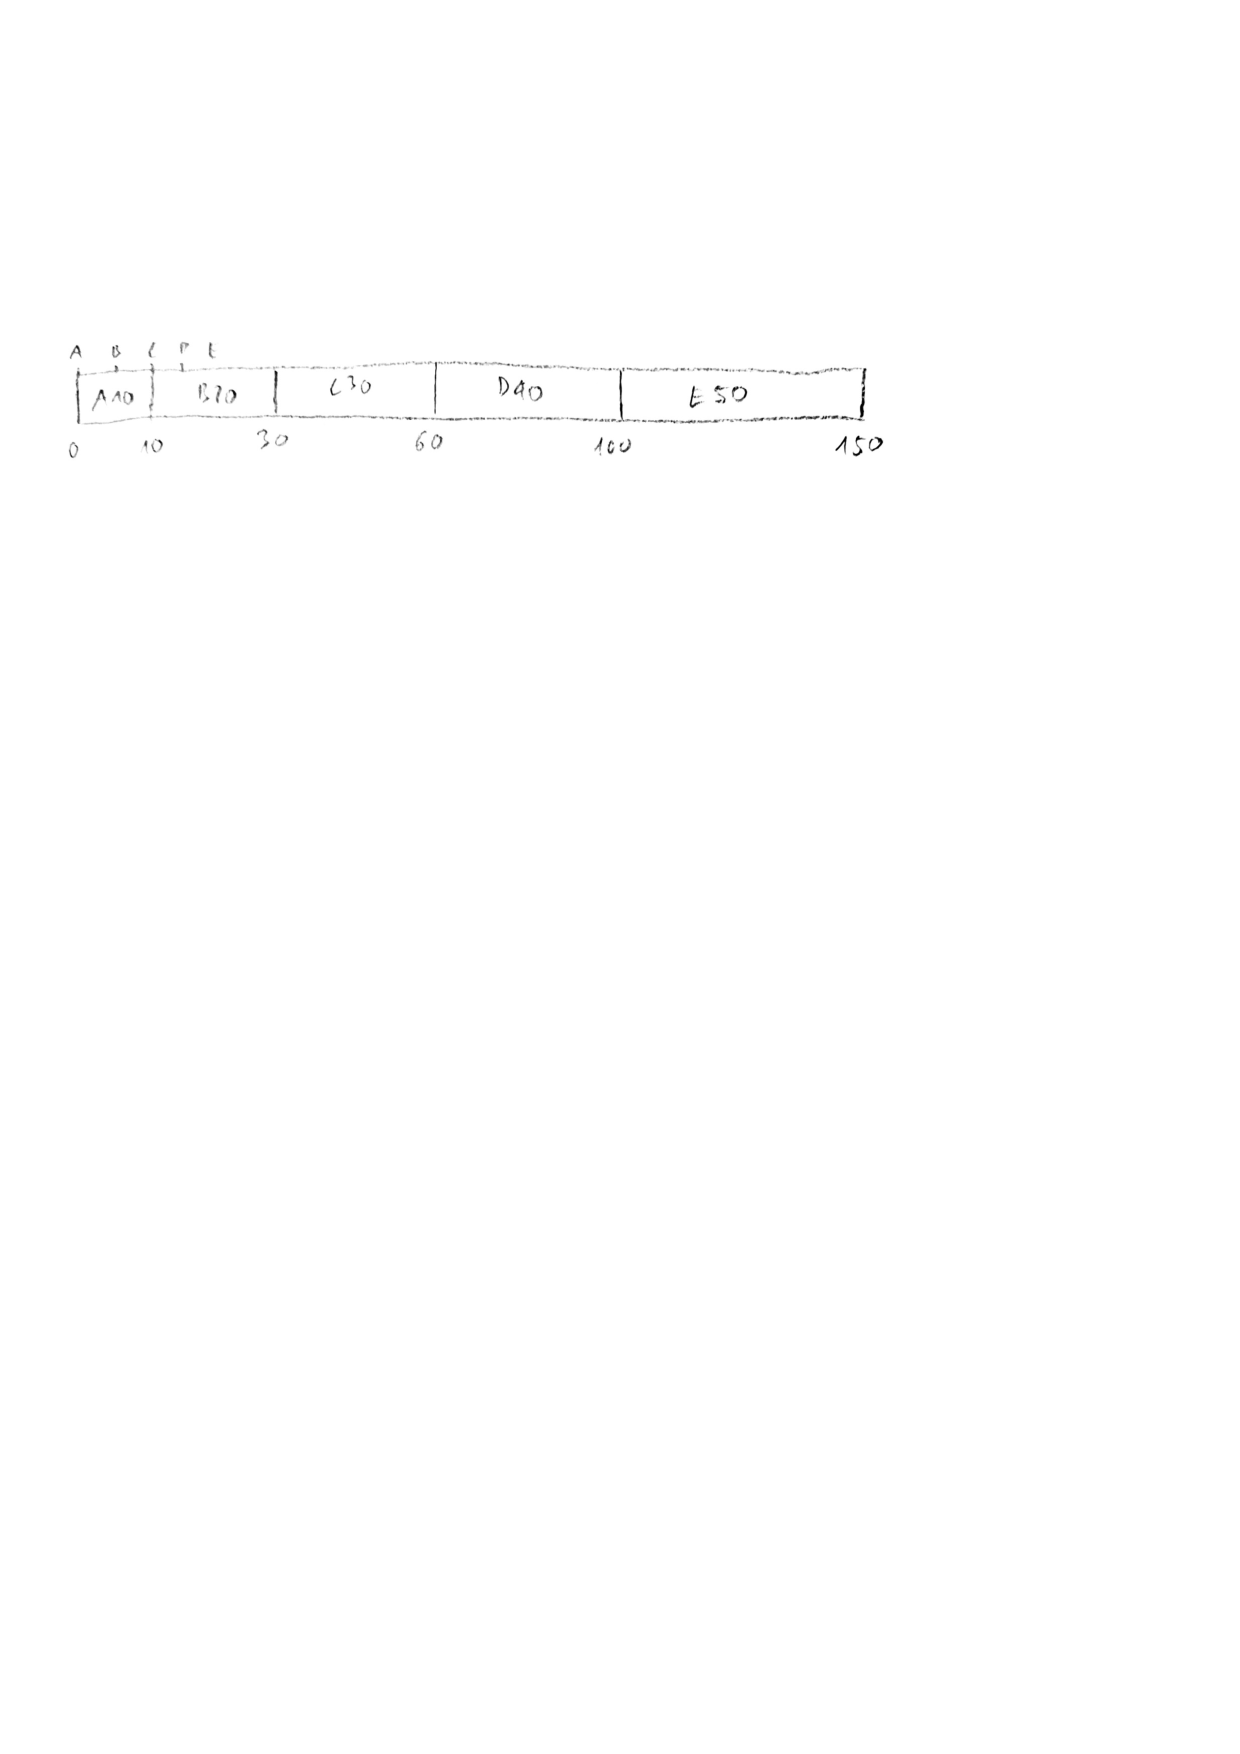
\includegraphics[width=.9\textwidth]{razvrscanje/1.1-FCFS,SJF.pdf}\\
\begin{tabular}{c|cc|cc|cc}
proces & trajanje & prihod & začetek & odhod & odzivni čas & čas obdelave \\
\hline
A & 10 &  0 &   0 & 10 & 0 & 10 \\
B & 20 &  5 & 10 & 30 & 5 & 25 \\
C & 30 & 10 & 30 & 60 & 20 & 50 \\
D & 40 & 15 & 60 & 100 & 45 & 85 \\
E & 50 & 20 & 100 & 150 & 80 & 130 \\
\hline
& & & & & 30 & 60
\end{tabular}
\end{center}
}


\begin{Exercise}
Za razvrščanje procesov v spodnji tabeli uporabi algoritma a) FCFS in b) SJF.
\par\vspace{5pt}
{\centering
\begin{tabular}{r|ccccc}
	proces & A & B & C & D & E \\
	\hline
	trajanje & 50 & 40 & 30 & 20 & 10 \\
	čas prihoda & 0 & 5 & 10 & 15 & 20 \\
\end{tabular}\\}
\end{Exercise}
\ans{
a) FCFS\\
\begin{center}
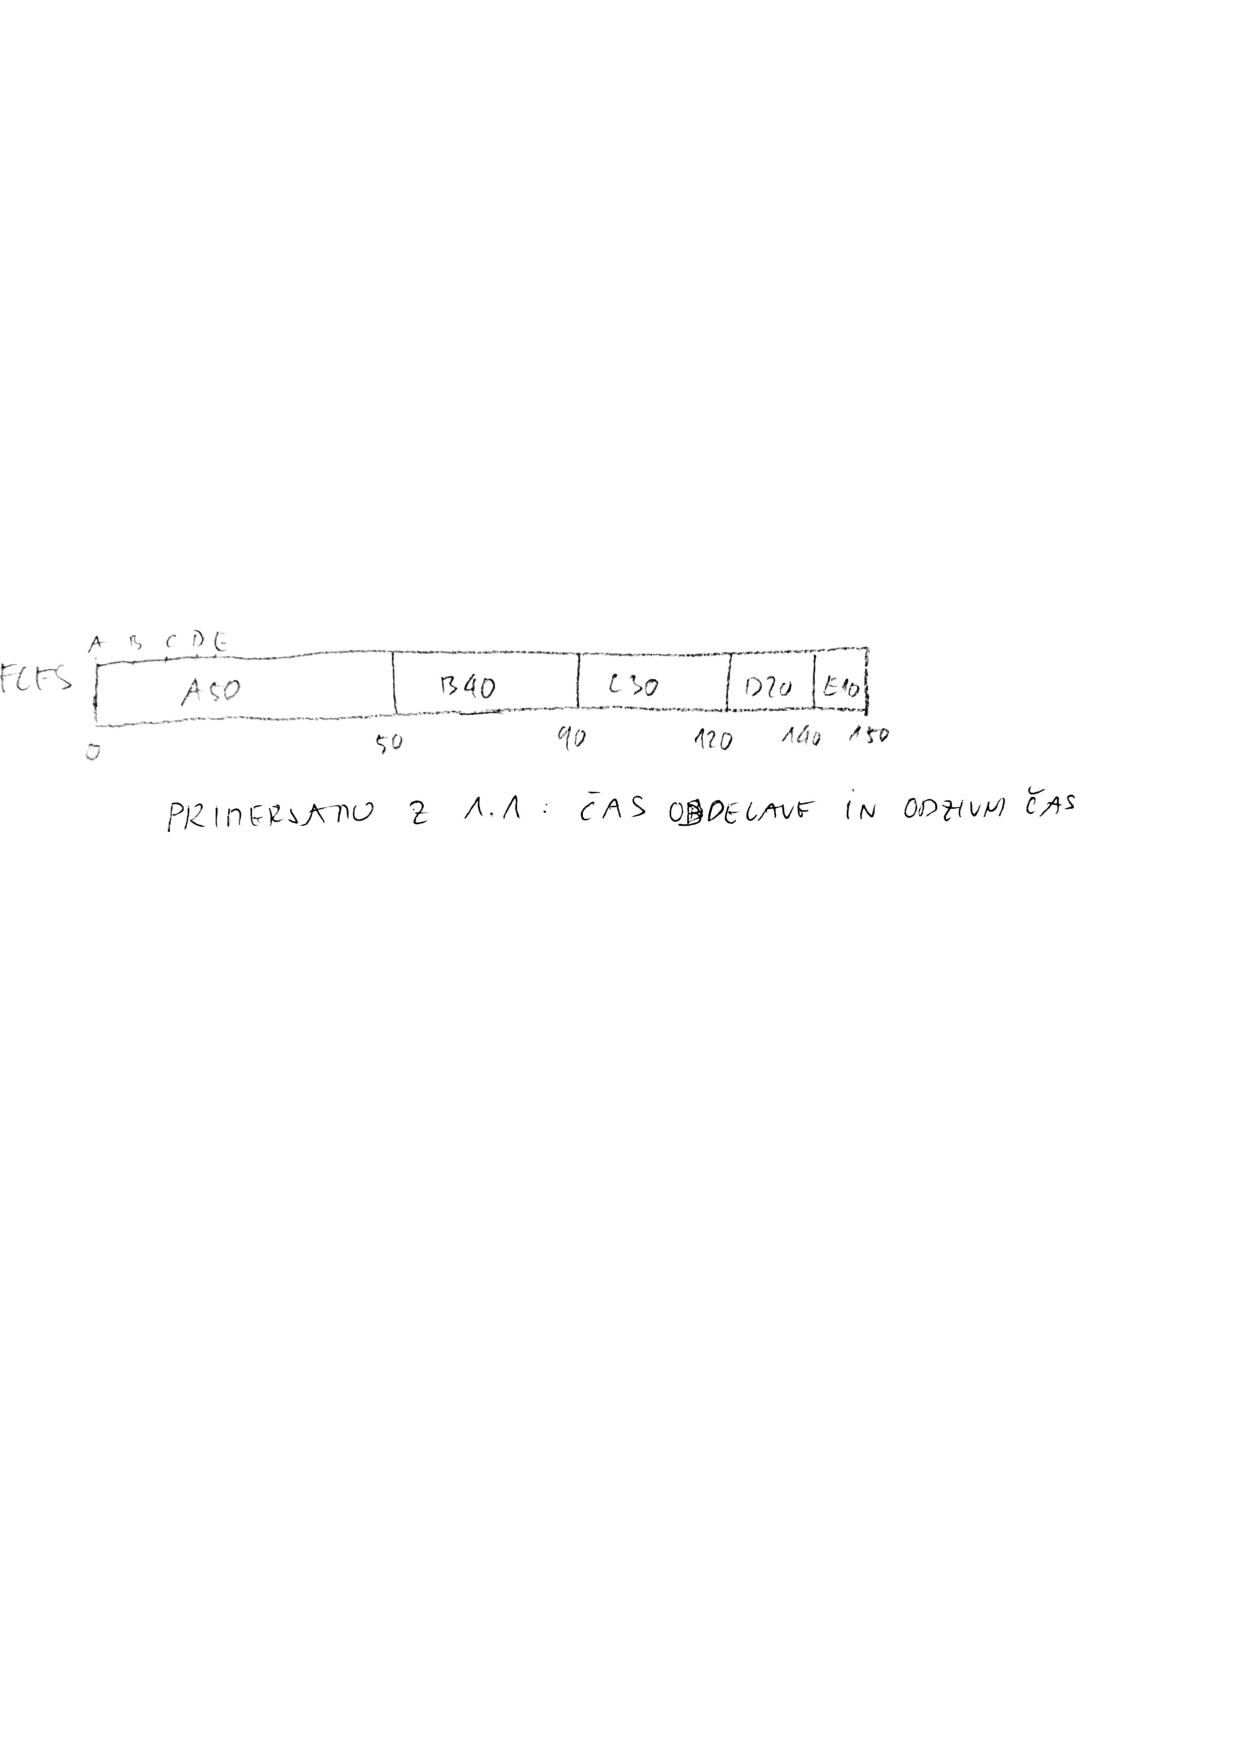
\includegraphics[width=.9\textwidth]{razvrscanje/1.2-FCFS.pdf}\\
\begin{tabular}{c|cc|cc|cc}
proces & trajanje & prihod & začetek & odhod & odzivni čas & čas obdelave \\
\hline
A & 50 &  0 &   0 & 50 & 0 & 50 \\
B & 40 &  5 & 50 & 90 & 45 & 85 \\
C & 30 & 10 & 90 & 120 & 80 & 110 \\
D & 20 & 15 & 120 & 140 & 105 & 125 \\
E & 10 & 20 & 140 & 150 & 120 & 130 \\
\hline
& & & & & 70 & 100
\end{tabular}
\end{center}
b) SJF:
\begin{center}
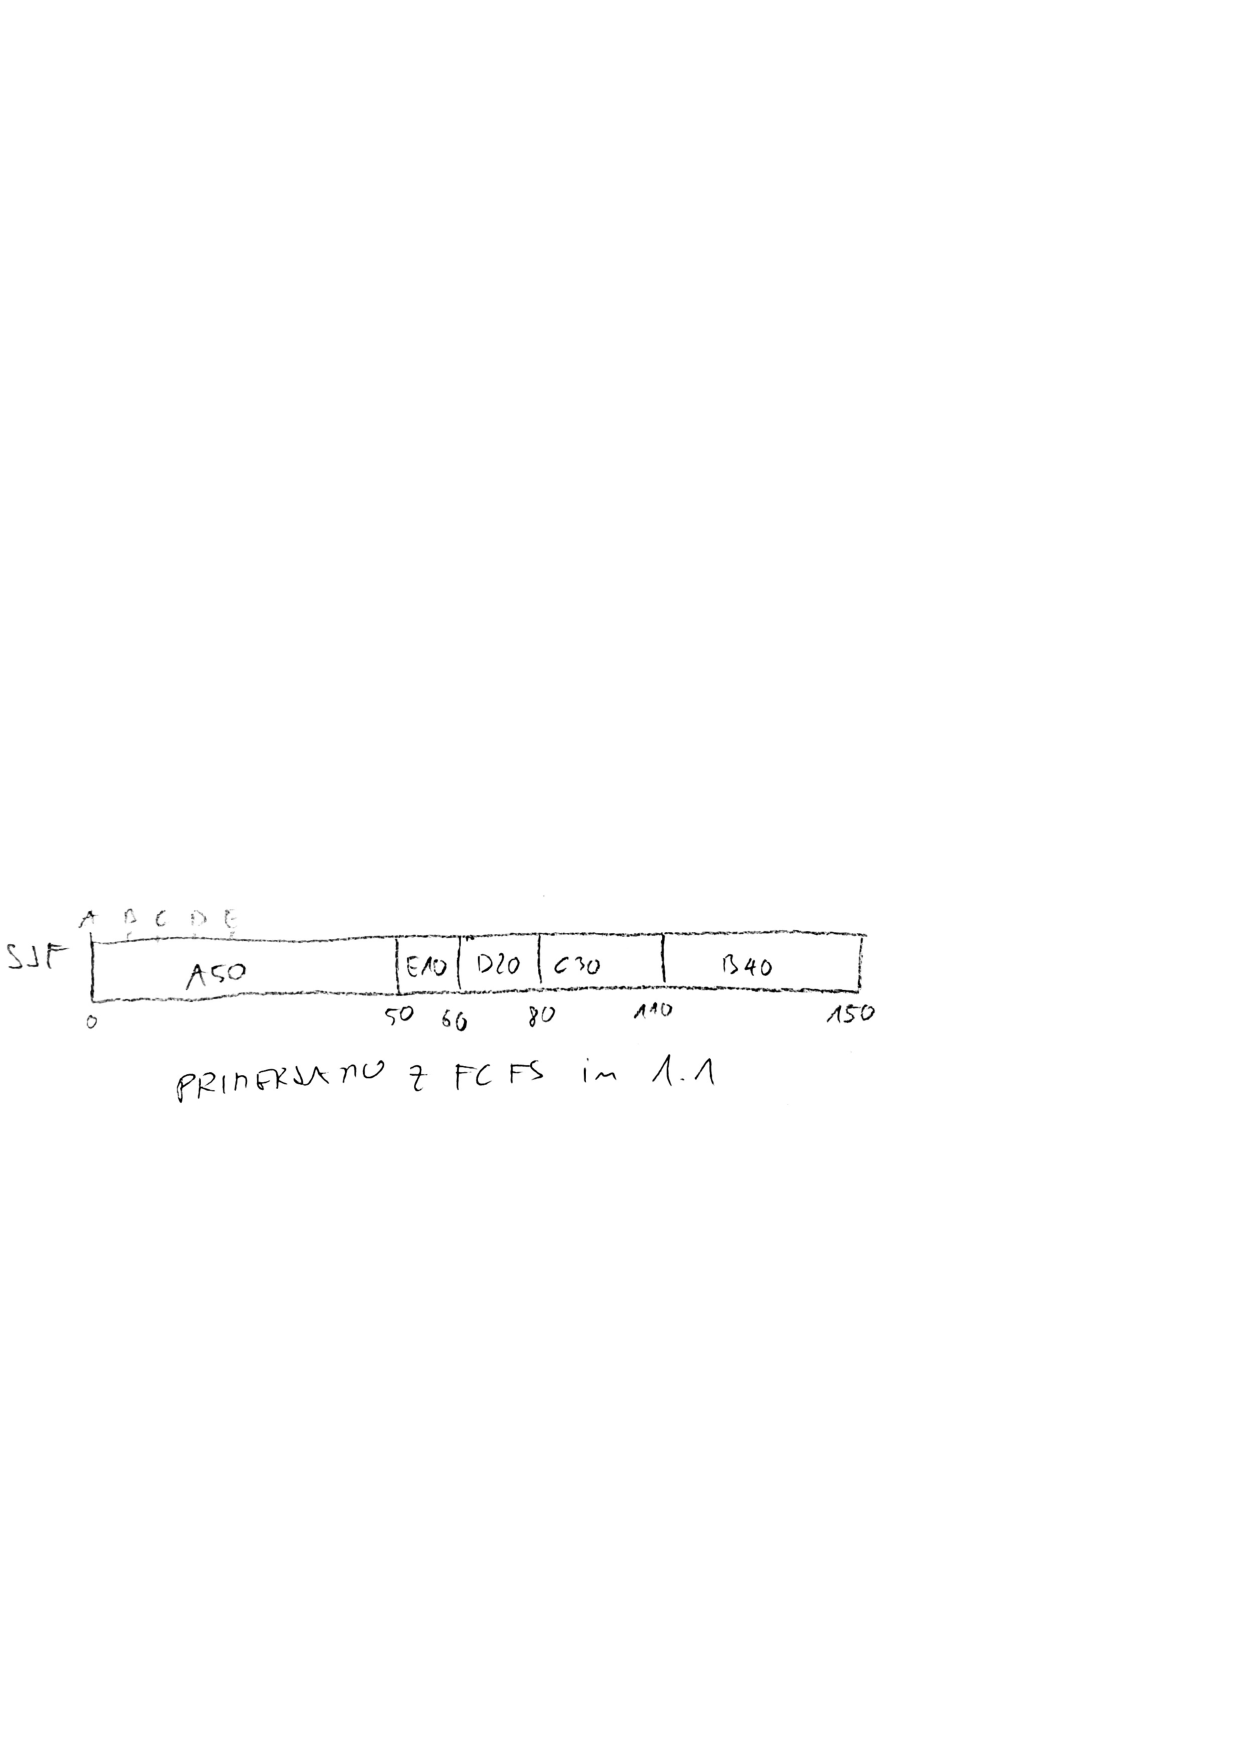
\includegraphics[width=.9\textwidth]{razvrscanje/1.2-SJF.pdf}\\
\begin{tabular}{c|cc|cc|cc}
proces & trajanje & prihod & začetek & odhod & odzivni čas & čas obdelave \\
\hline
A & 50 &  0 &   0 & 50 & 0 & 50 \\
B & 40 &  5 & 110 & 150 & 105 & 145 \\
C & 30 & 10 & 80 & 110 & 70 & 100 \\
D & 20 & 15 & 60 & 80 & 45 & 65 \\
E & 10 & 20 & 50 & 60 & 30 & 40 \\
\hline
& & & & & 50 & 80
\end{tabular}
\end{center}
}


\begin{Exercise}
Za razvrščanje procesov v spodnji tabeli uporabi algoritma a) FCFS in b) SJF.
\par\vspace{5pt}
{\centering
\begin{tabular}{r|ccccc}
	proces & A & B & C & D & E \\
	\hline
	trajanje & 10 & 30 & 30 & 10 & 20 \\
	čas prihoda & 0 & 0 & 10 & 10 & 20 \\
\end{tabular}\\}
\end{Exercise}
\ans{
a) FCFS:
\begin{center}
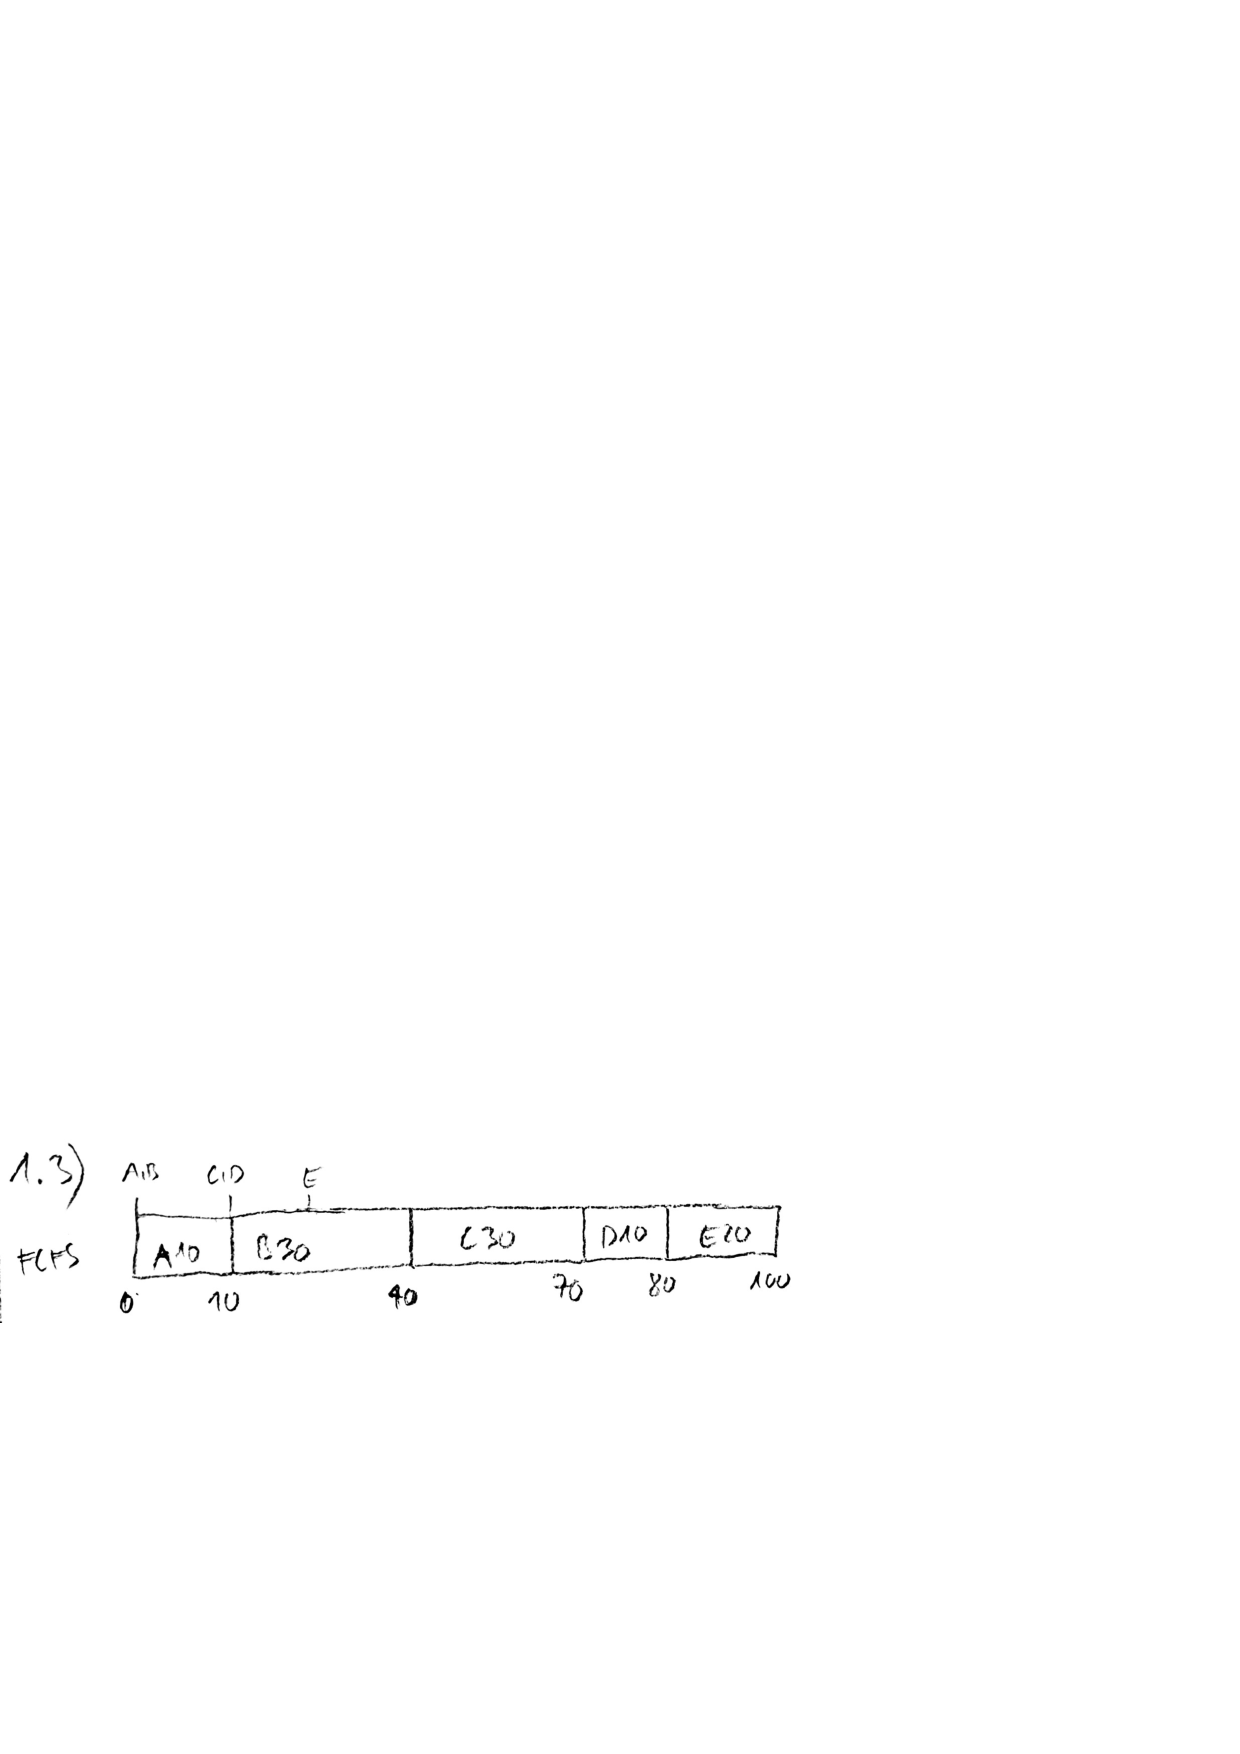
\includegraphics[width=.9\textwidth]{razvrscanje/1.3-FCFS.pdf}\\
\begin{tabular}{c|cc|cc|cc}
proces & trajanje & prihod & začetek & odhod & odzivni čas & čas obdelave \\
\hline
A & 10 &  0 &   0 & 10 & 0 & 10 \\
B & 30 &  0 & 10 & 40 & 10 & 40 \\
C & 30 & 10 & 40 & 70 & 30 & 60 \\
D & 10 & 10 & 70 & 80 & 60 & 70 \\
E & 20 & 20 & 80 & 100 & 60 & 80 \\
\hline
& & & & & 32 & 52
\end{tabular}
\end{center}
b) SJF:
\begin{center}
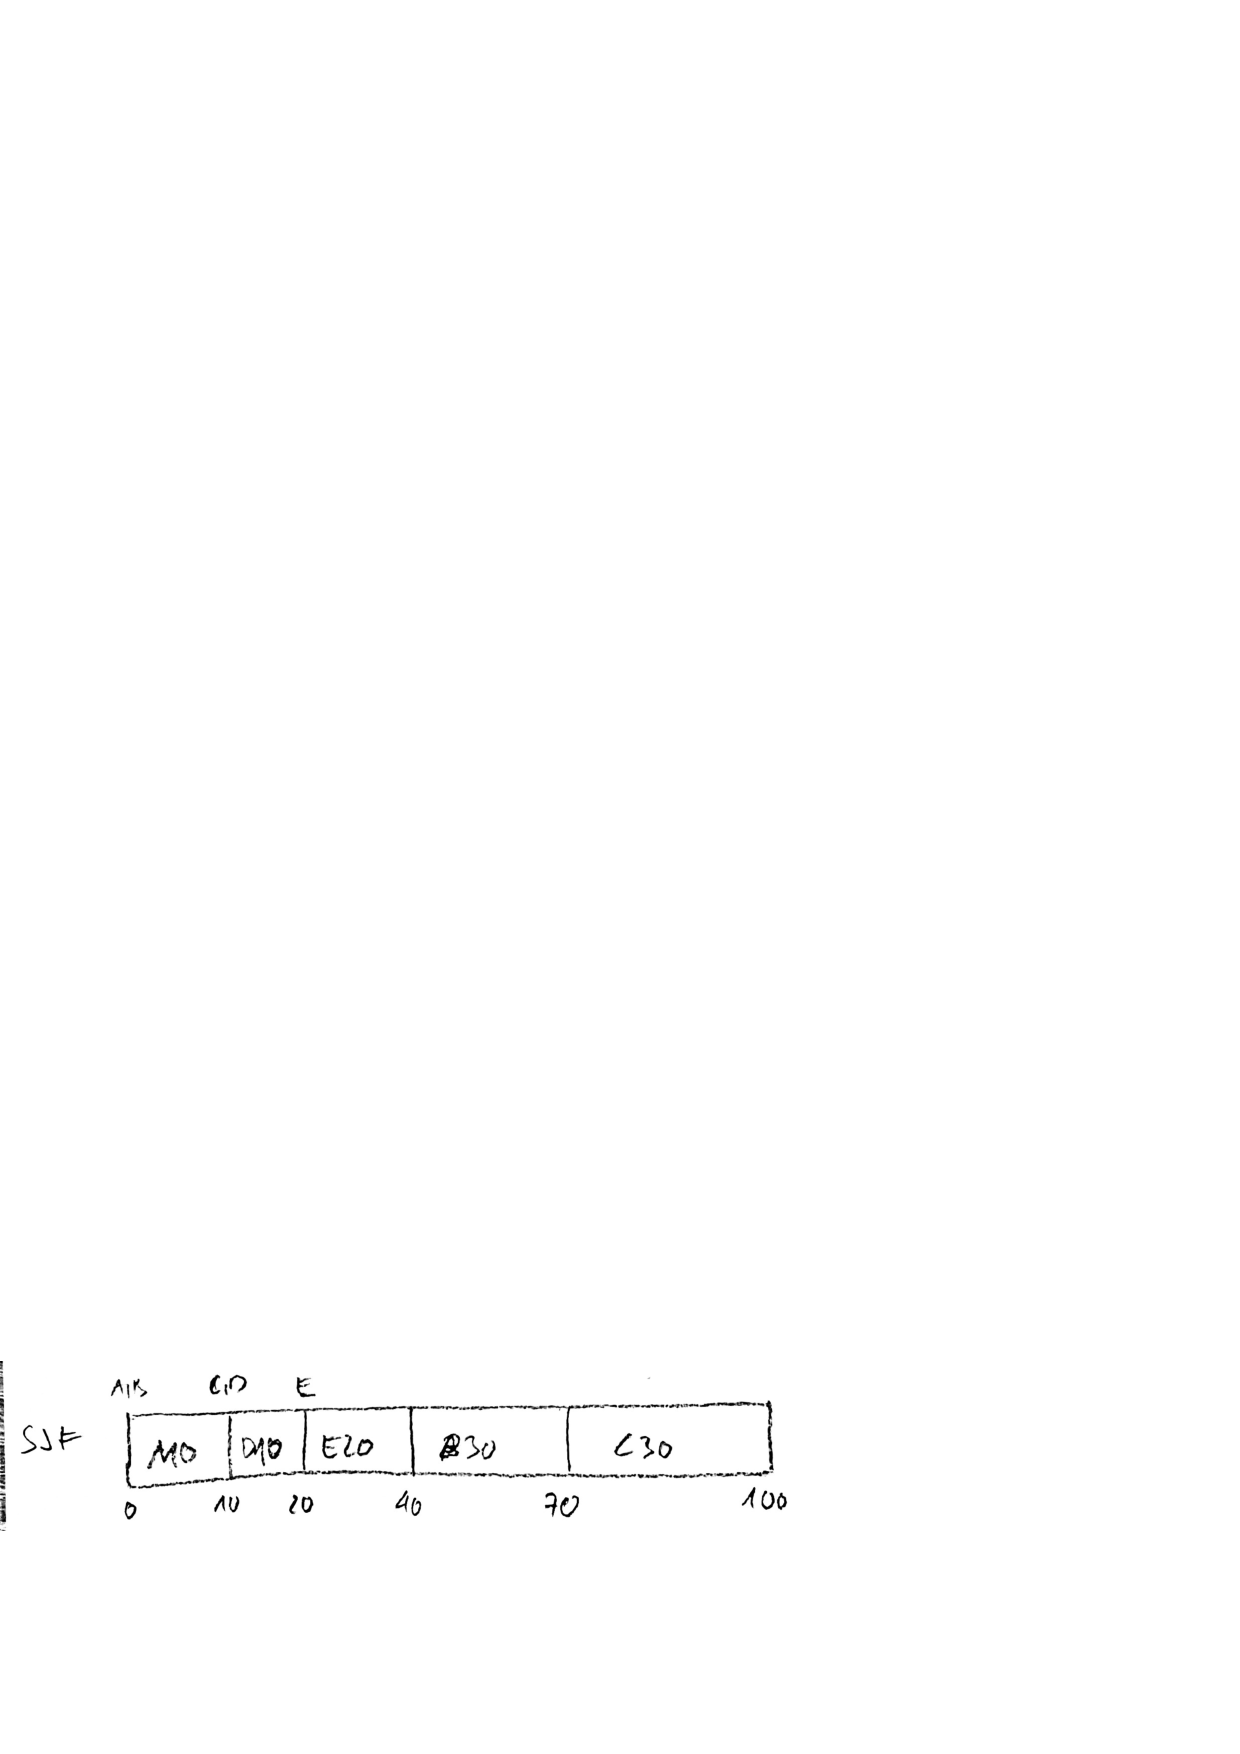
\includegraphics[width=.9\textwidth]{razvrscanje/1.3-SJF.pdf}\\
\begin{tabular}{c|cc|cc|cc}
proces & trajanje & prihod & začetek & odhod & odzivni čas & čas obdelave \\
\hline
A & 10 &  0 &   0 & 10 & 0 & 10 \\
B & 30 &  0 & 40 & 70 & 40 & 70  \\
C & 30 & 10 & 70 & 100 & 60 & 90 \\
D & 10 & 10 & 10 & 20 & 0 & 10 \\
E & 20 & 20 & 20 & 40 & 0 & 20 \\
\hline
& & & & & 20 & 40
\end{tabular}
\end{center}
}


\begin{Exercise}
Za razvrščanje procesov v spodnji tabeli uporabi algoritma a) SJF in b) PSJF.
\par\vspace{5pt}
{\centering
	\begin{tabular}{r|ccccc}
		proces & A & B & C & D & E \\
		\hline
		trajanje & 25 & 10 & 15 & 10 & 5 \\
		čas prihoda & 0 & 5 & 10 & 15 & 30 \\
	\end{tabular}\\}
\end{Exercise}
\ans{
a) SJF:
\begin{center}
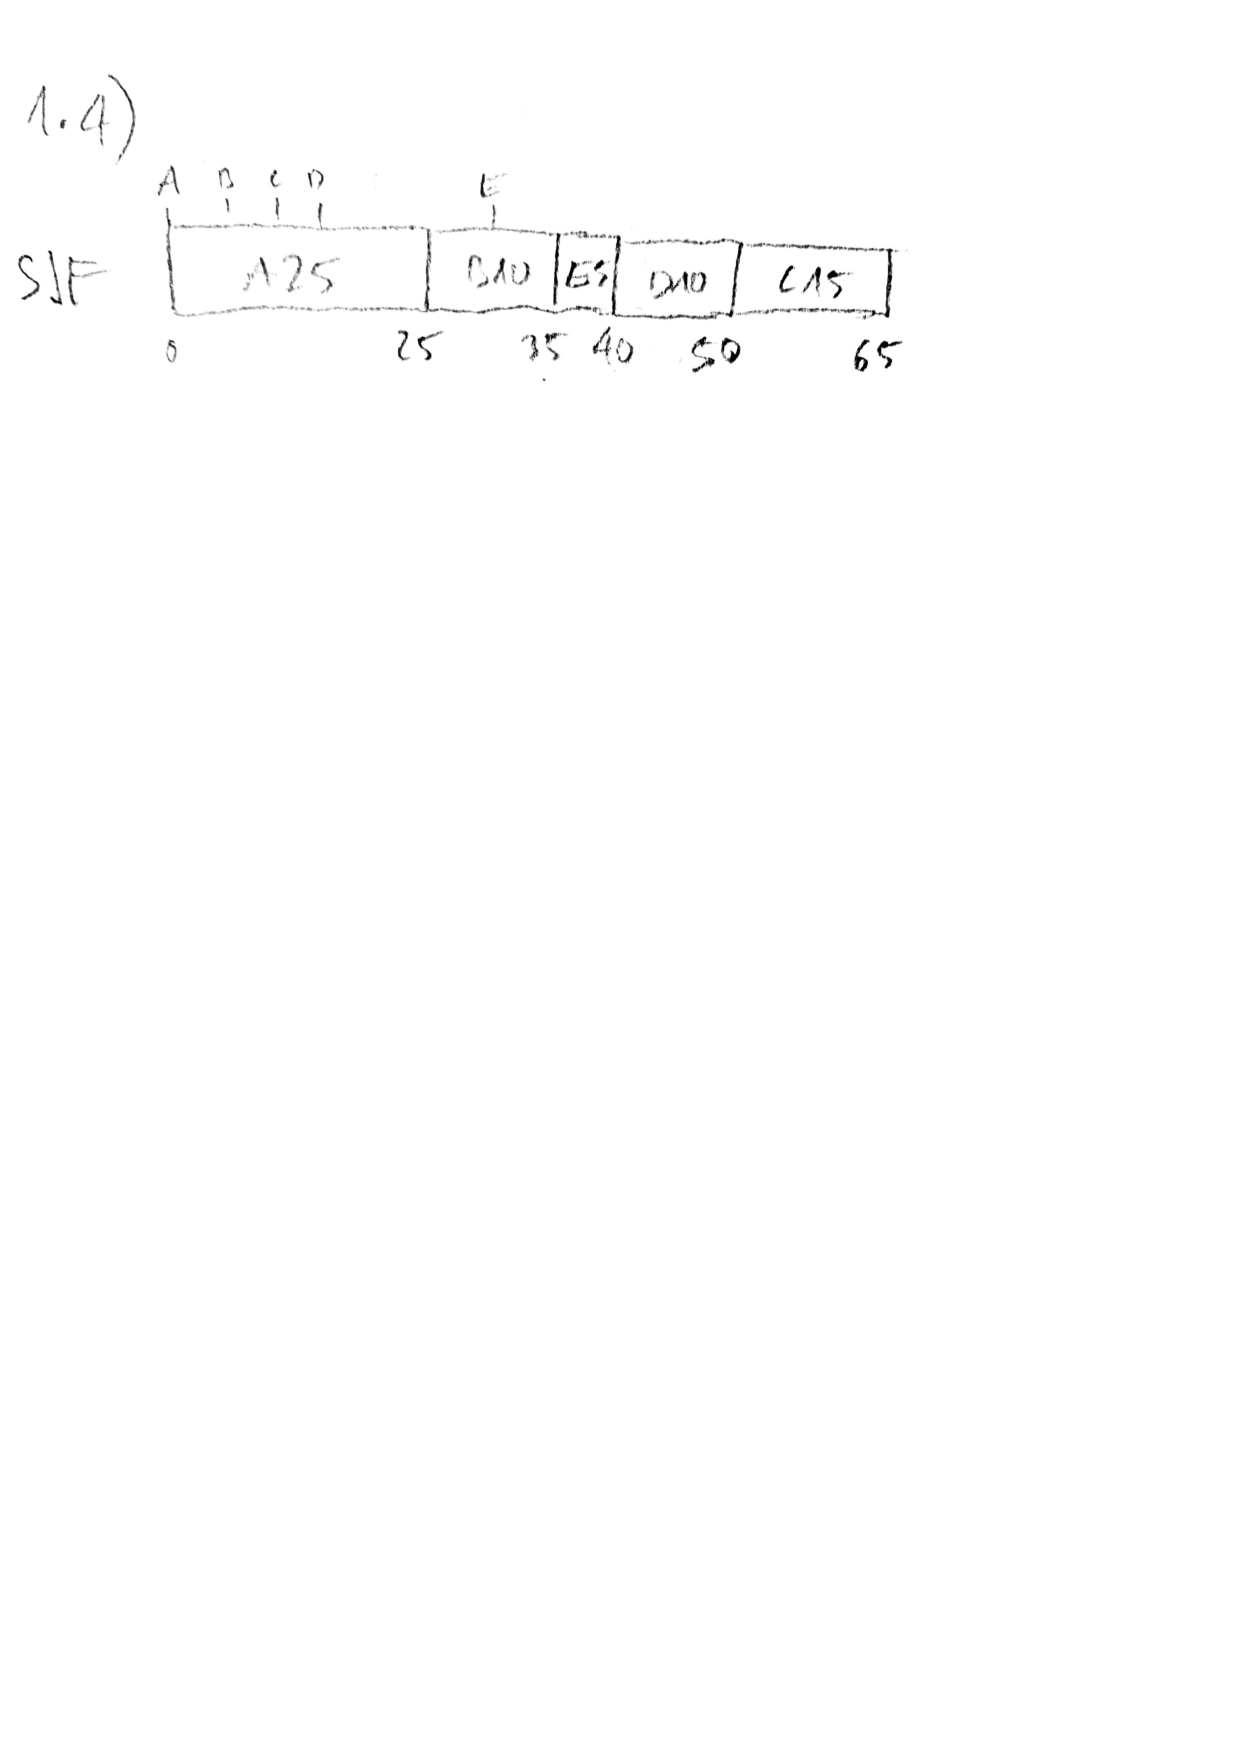
\includegraphics[width=.8\textwidth]{razvrscanje/1.4-SJF.pdf}\\
\begin{tabular}{c|cc|cc|cc}
proces & trajanje & prihod & začetek & odhod & odzivni čas & čas obdelave \\
\hline
A & 25 &  0 &   0 & 25 & 0 & 25 \\
B & 10 &  5 & 25 & 35 & 20 & 30 \\
C & 15 & 10 & 50 & 65 & 40 & 55 \\
D & 10 & 15 & 40 & 50 & 25 & 35 \\
E &  5 & 30 & 35 & 40 & 5 & 10 \\
\hline
& & & & & 18 & 31
\end{tabular}
\end{center}
b) PSJF:
\begin{center}
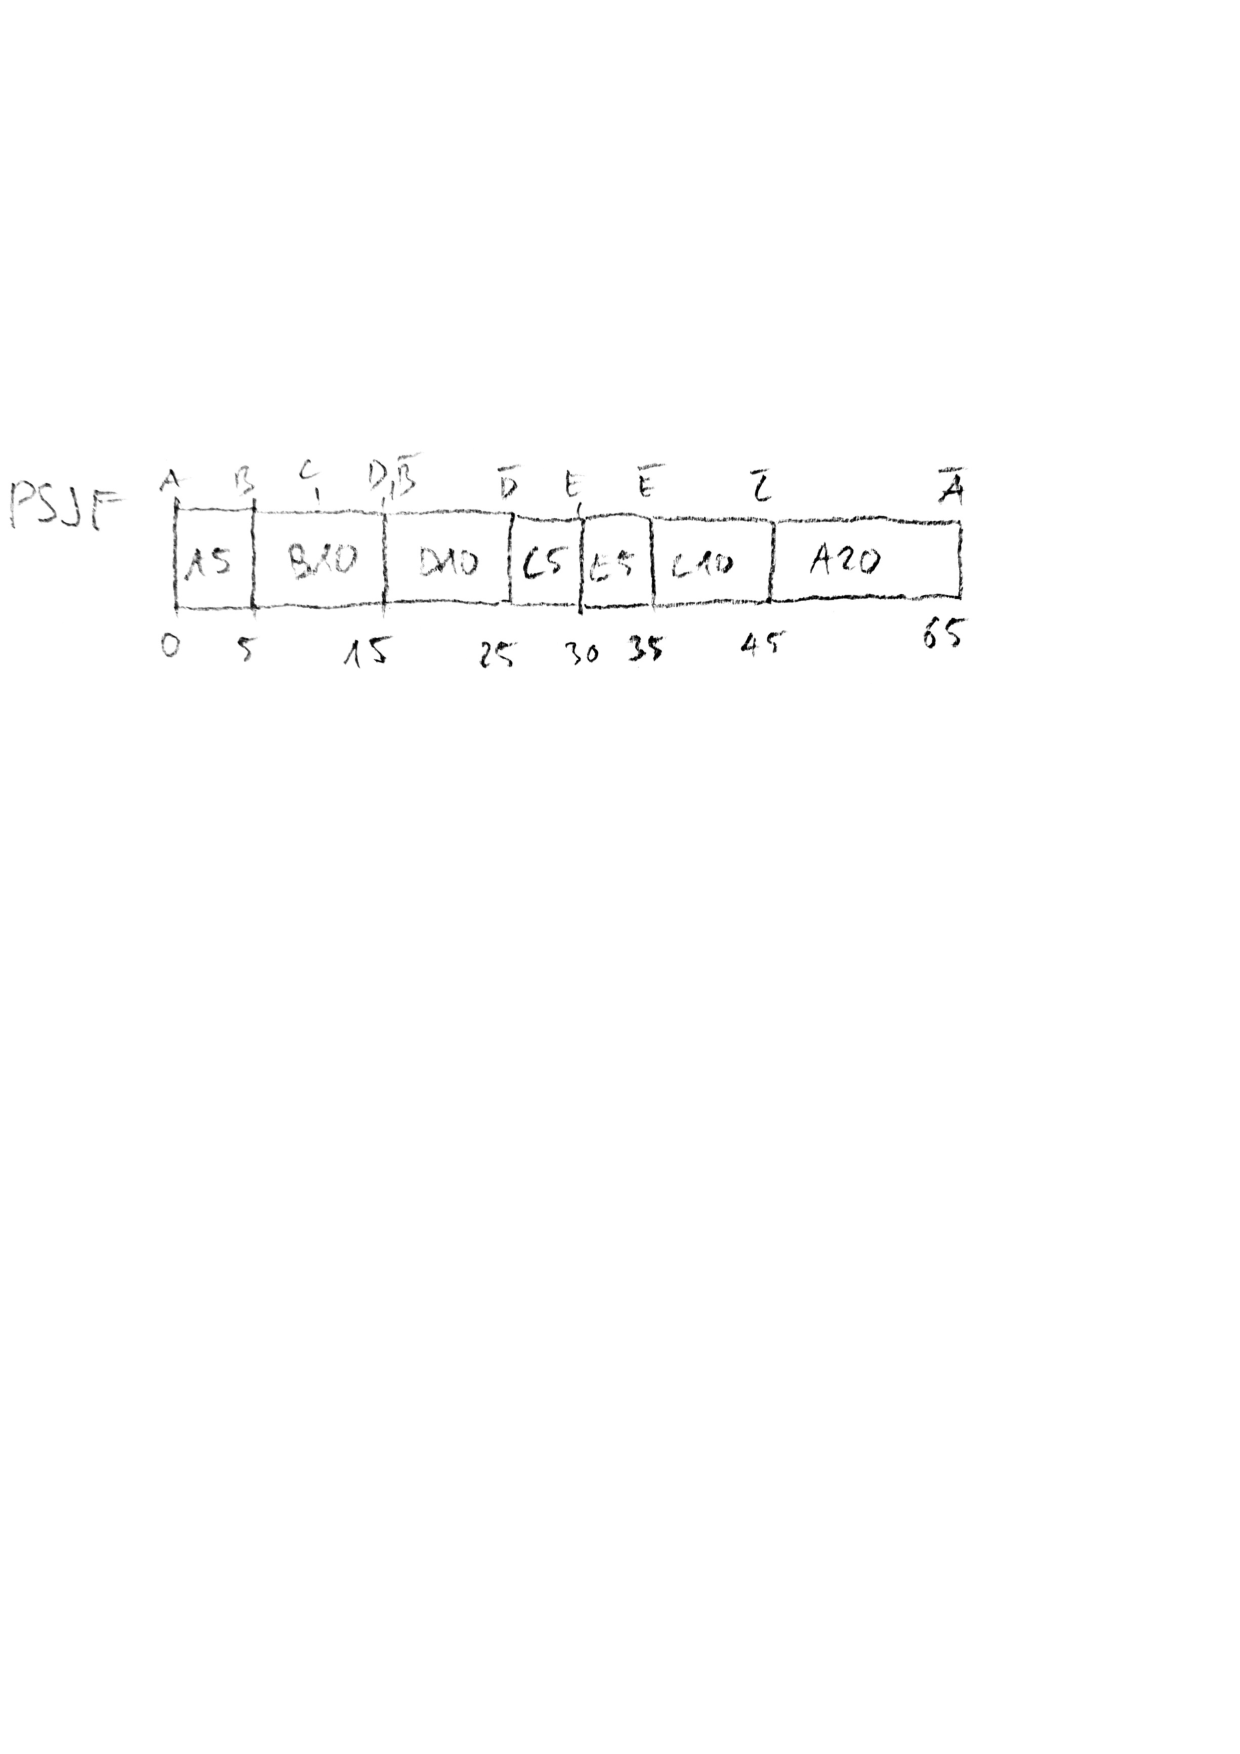
\includegraphics[width=.8\textwidth]{razvrscanje/1.4-PSJF.pdf}\\
\begin{tabular}{c|cc|cc|cc}
proces & trajanje & prihod & začetek & odhod & odzivni čas & čas obdelave \\
\hline
A & 25 &  0 &   0 & 65 & 0 & 65 \\
B & 10 &  5 &   5 & 15 &  0 & 10 \\
C & 15 & 10 & 25 & 45 & 15 & 35 \\
D & 10 & 15 & 15 & 25 & 0 & 10 \\
E &  5 & 30 & 30 & 35 & 0 & 5 \\
\hline
& & & & & 3 & 25
\end{tabular}
\end{center}
}


\begin{Exercise}
Za razvrščanje procesov v spodnji tabeli uporabi algoritem RR. Pri tem uporabi časovno rezino: a) 10 časovnih enot in b) 5 časovnih enot.
\par\vspace{5pt}
{\centering
\begin{tabular}{r|ccc}
	proces & A & B & C \\
	\hline
	trajanje & 15 & 10 & 5  \\
	čas prihoda & 0 & 5 & 5 \\
\end{tabular}\\}
\end{Exercise}
\ans{
Narišemo le diagrama za obe časovni rezini.
\begin{center}
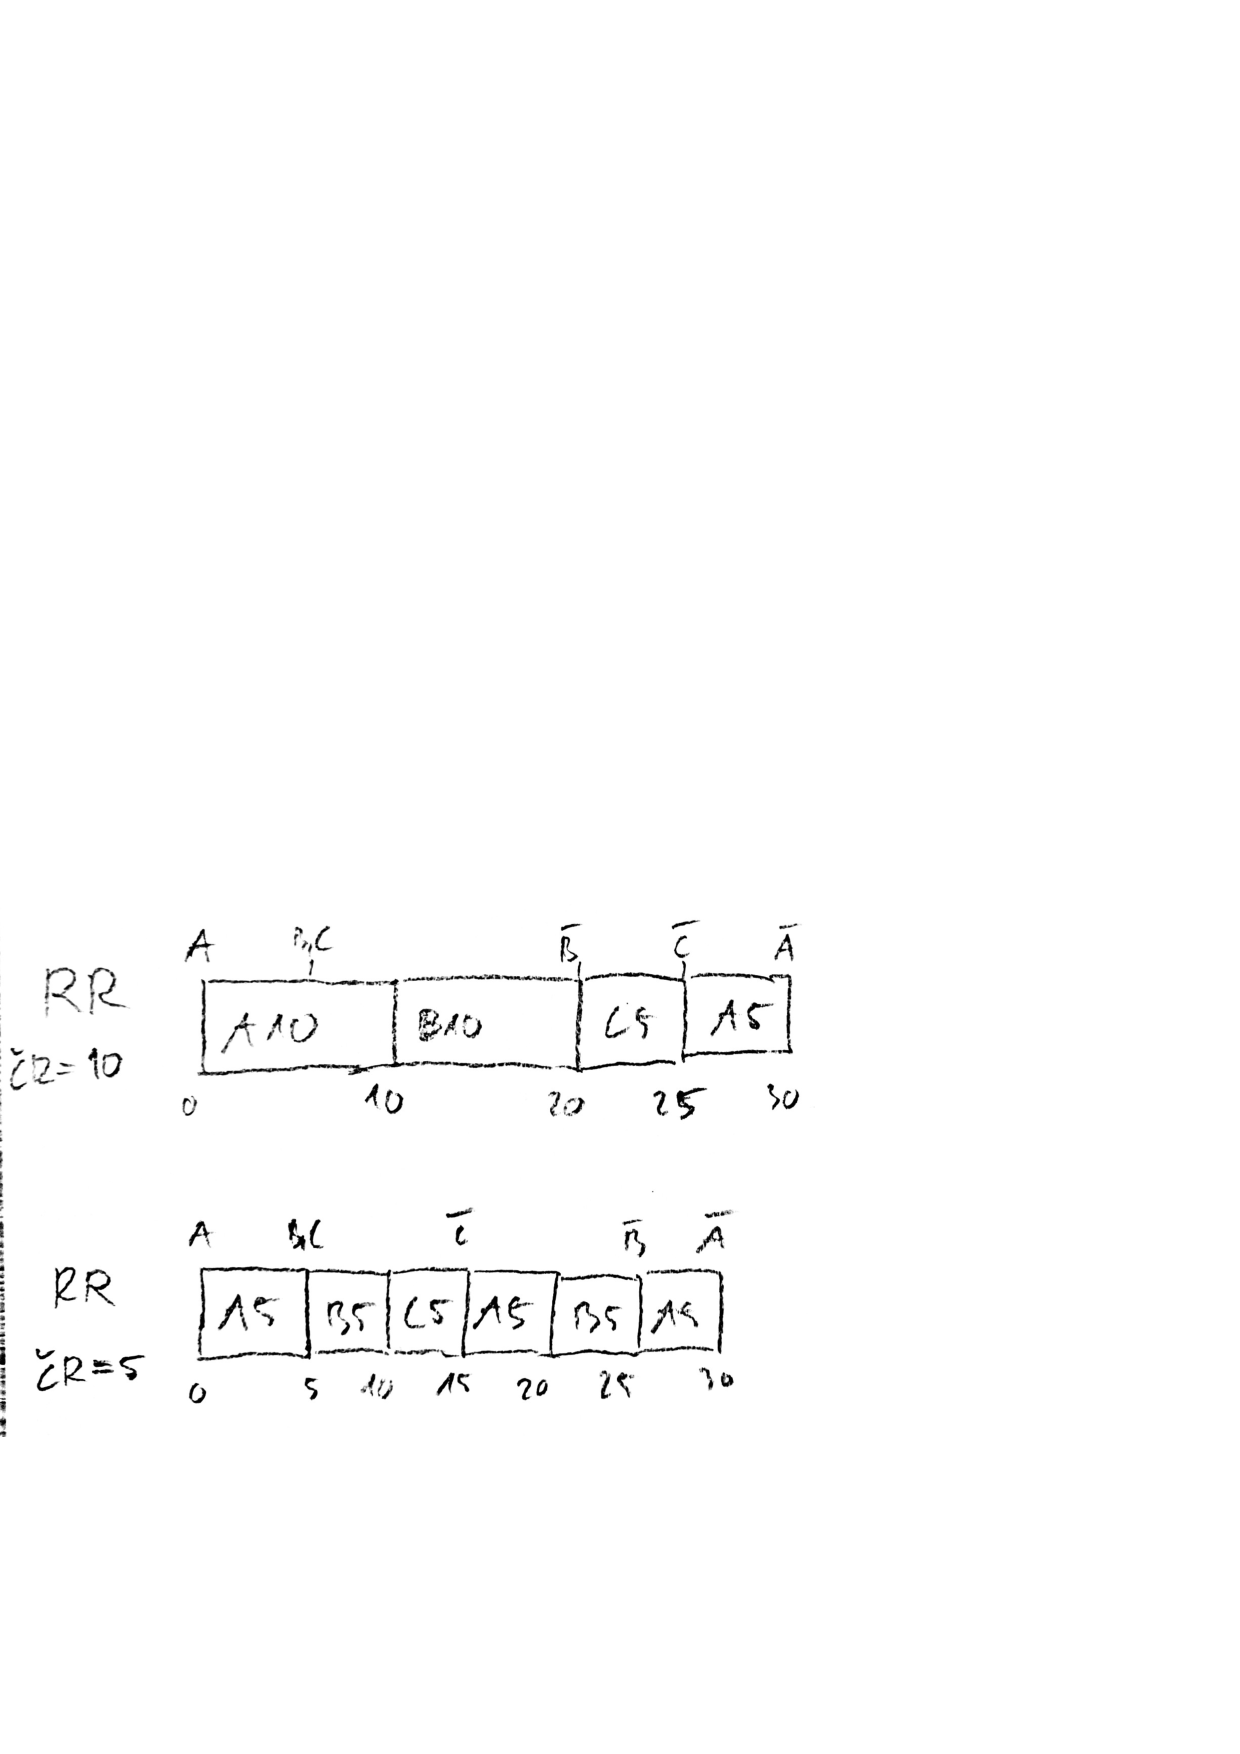
\includegraphics[width=.6\textwidth]{razvrscanje/1.5-RR.pdf}
\end{center}
}


\section{Efekt konvoja}

\intro{Naslednji dve nalogi sta namenjeni razlagi efekta konvoja na čas obdelave.}

\begin{Exercise}
Za razvrščanje procesov v dani tabeli uporabi optimalno razvrstitev glede na čas obdelave.
\par\vspace{5pt}
{\centering
\begin{tabular}{r|cccc}
	proces & A & B & C & D \\
	\hline
	trajanje & 7 & 2 & 19 & 6  \\
	čas prihoda & 0 & 0 & 0 & 0 \\
\end{tabular}\\}
\end{Exercise}
\ans{
OPT je SJF.
\begin{center}
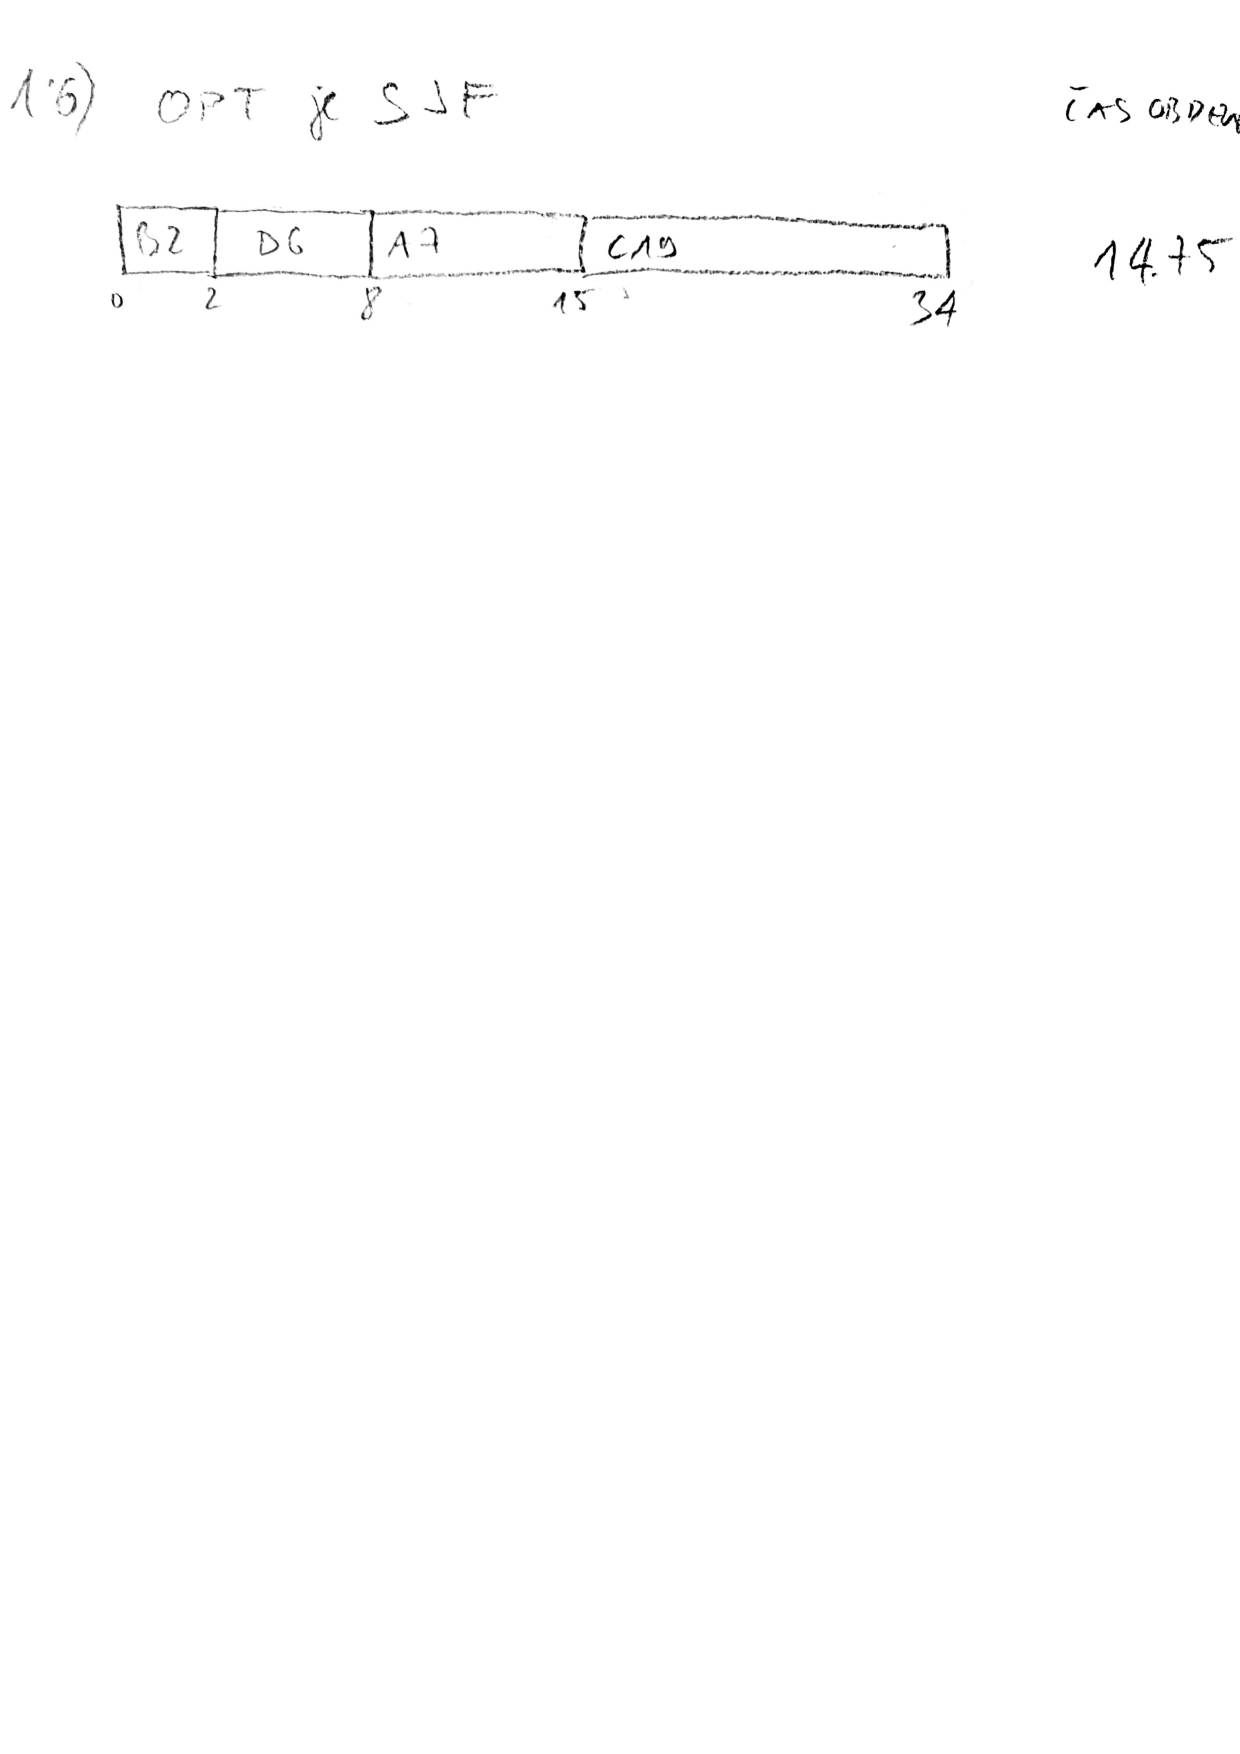
\includegraphics[width=.9\textwidth]{razvrscanje/1.6-OPT.pdf}\\
\begin{tabular}{c|cc|cc|cc}
proces & trajanje & prihod & začetek & odhod & odzivni čas & čas obdelave \\
\hline
A &   7 &  0 & 8 & 15 & 8 & 15 \\
B &   2 &  0 & 0 & 2 & 0 & 2 \\
C & 19 & 0 & 15 & 34 & 15 & 34 \\
D &   6 & 0 & 2 & 8 & 2 & 8 \\
\hline
& & & & & 6,25 & 14,75
\end{tabular}
\end{center}
}


\begin{Exercise}
Za razvrščanje procesov v dani tabeli uporabi algoritme FCFS, SJF in PSJF. V primeru dvoumnosti glede časa prihoda, procese razvrstimo leksikografsko.
\par\vspace{5pt}
{\centering
\begin{tabular}{r|cccc}
	proces & A & B & C & D \\
	\hline
	trajanje & 7 & 2 & 19 & 6  \\
	čas prihoda & 1 & 1 & 0 & 1 \\
\end{tabular}\\}
\end{Exercise}
\ans{
FCFS:
\begin{center}
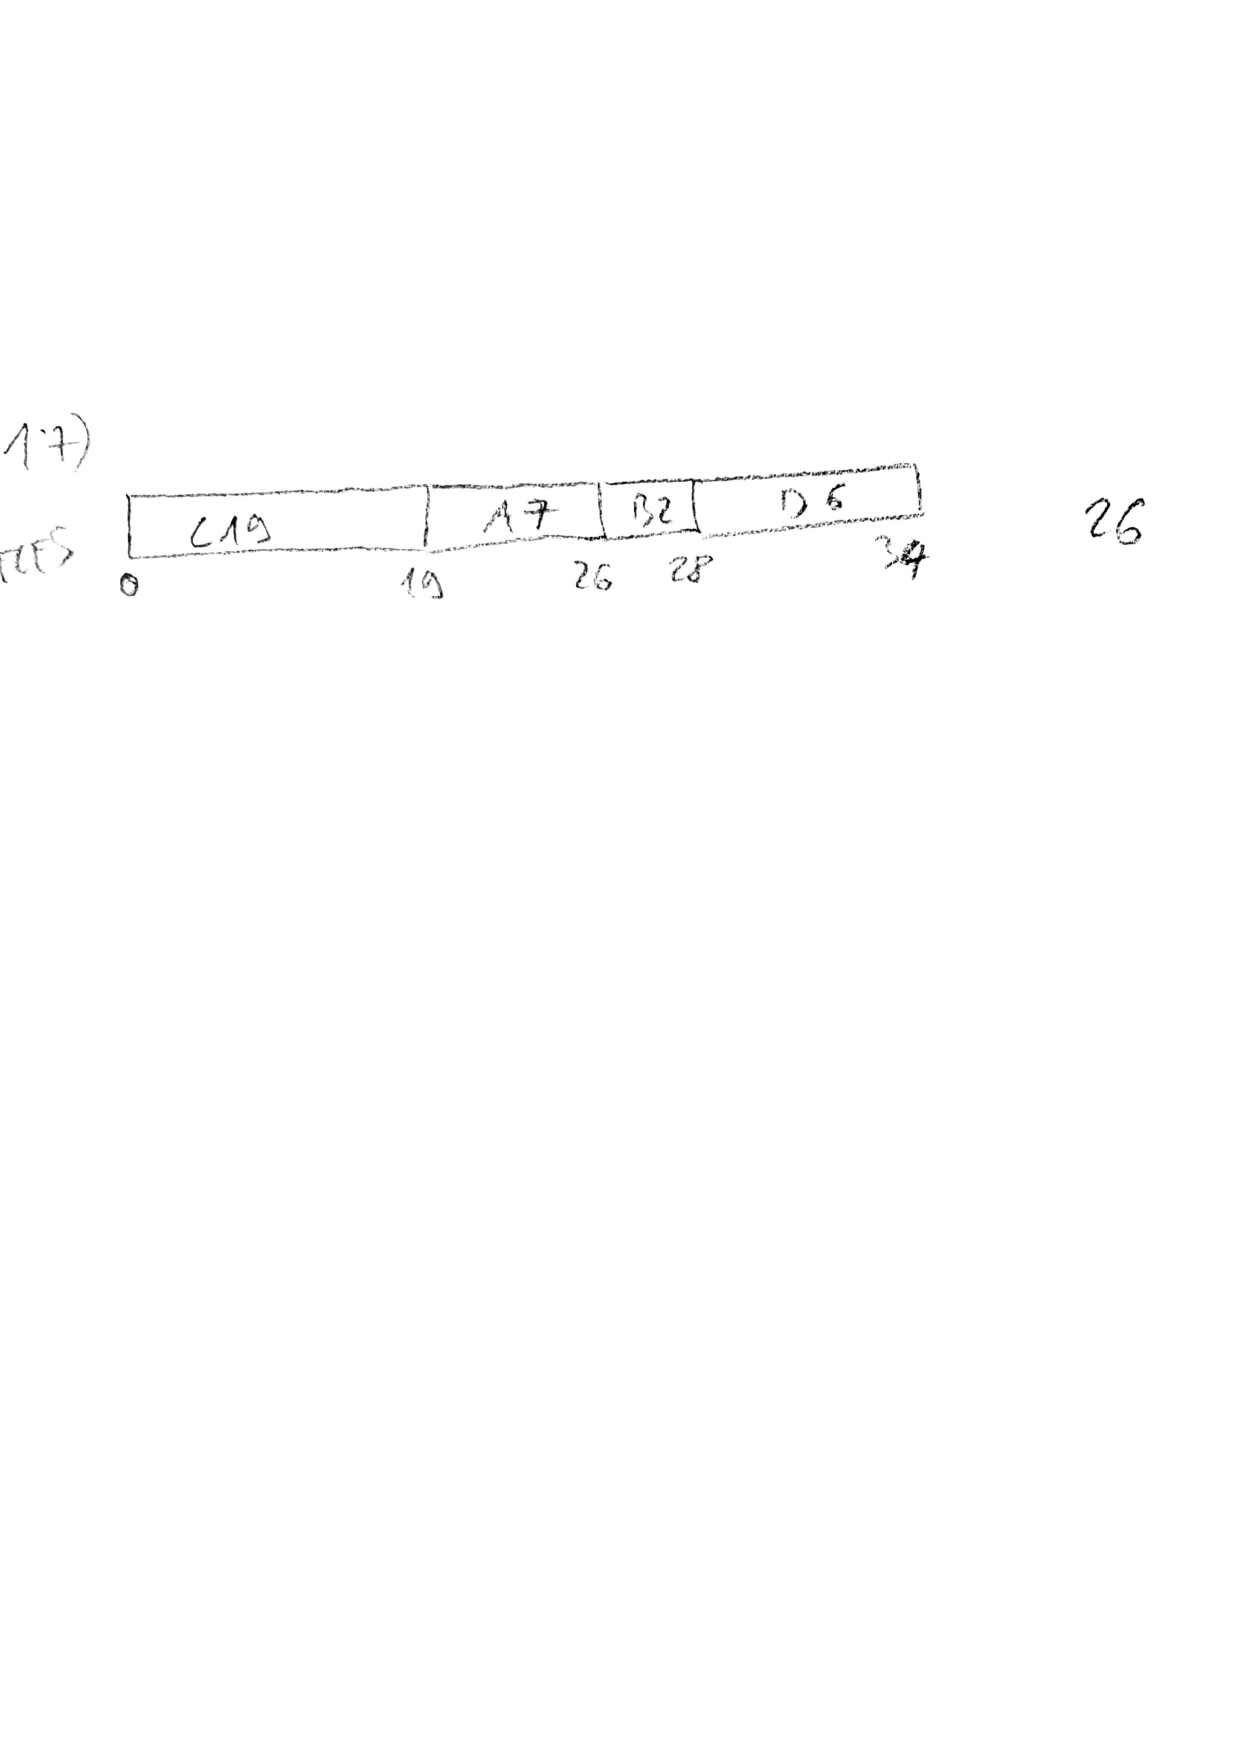
\includegraphics[width=.9\textwidth]{razvrscanje/1.7-FCFS.pdf}\\
\begin{tabular}{c|cc|cc|cc}
proces & trajanje & prihod & začetek & odhod & odzivni čas & čas obdelave \\
\hline
A &   7 &  1 & 19 & 26 & 18 & 25 \\
B &   2 &  1 & 26 & 28 & 25 & 27 \\
C & 19 & 0 &  0 & 19 & 0 & 19 \\
D &   6 & 1 & 28 & 34 & 27 & 33 \\
\hline
& & & & & 17,5 & 26
\end{tabular}
\end{center}
SJF:
\begin{center}
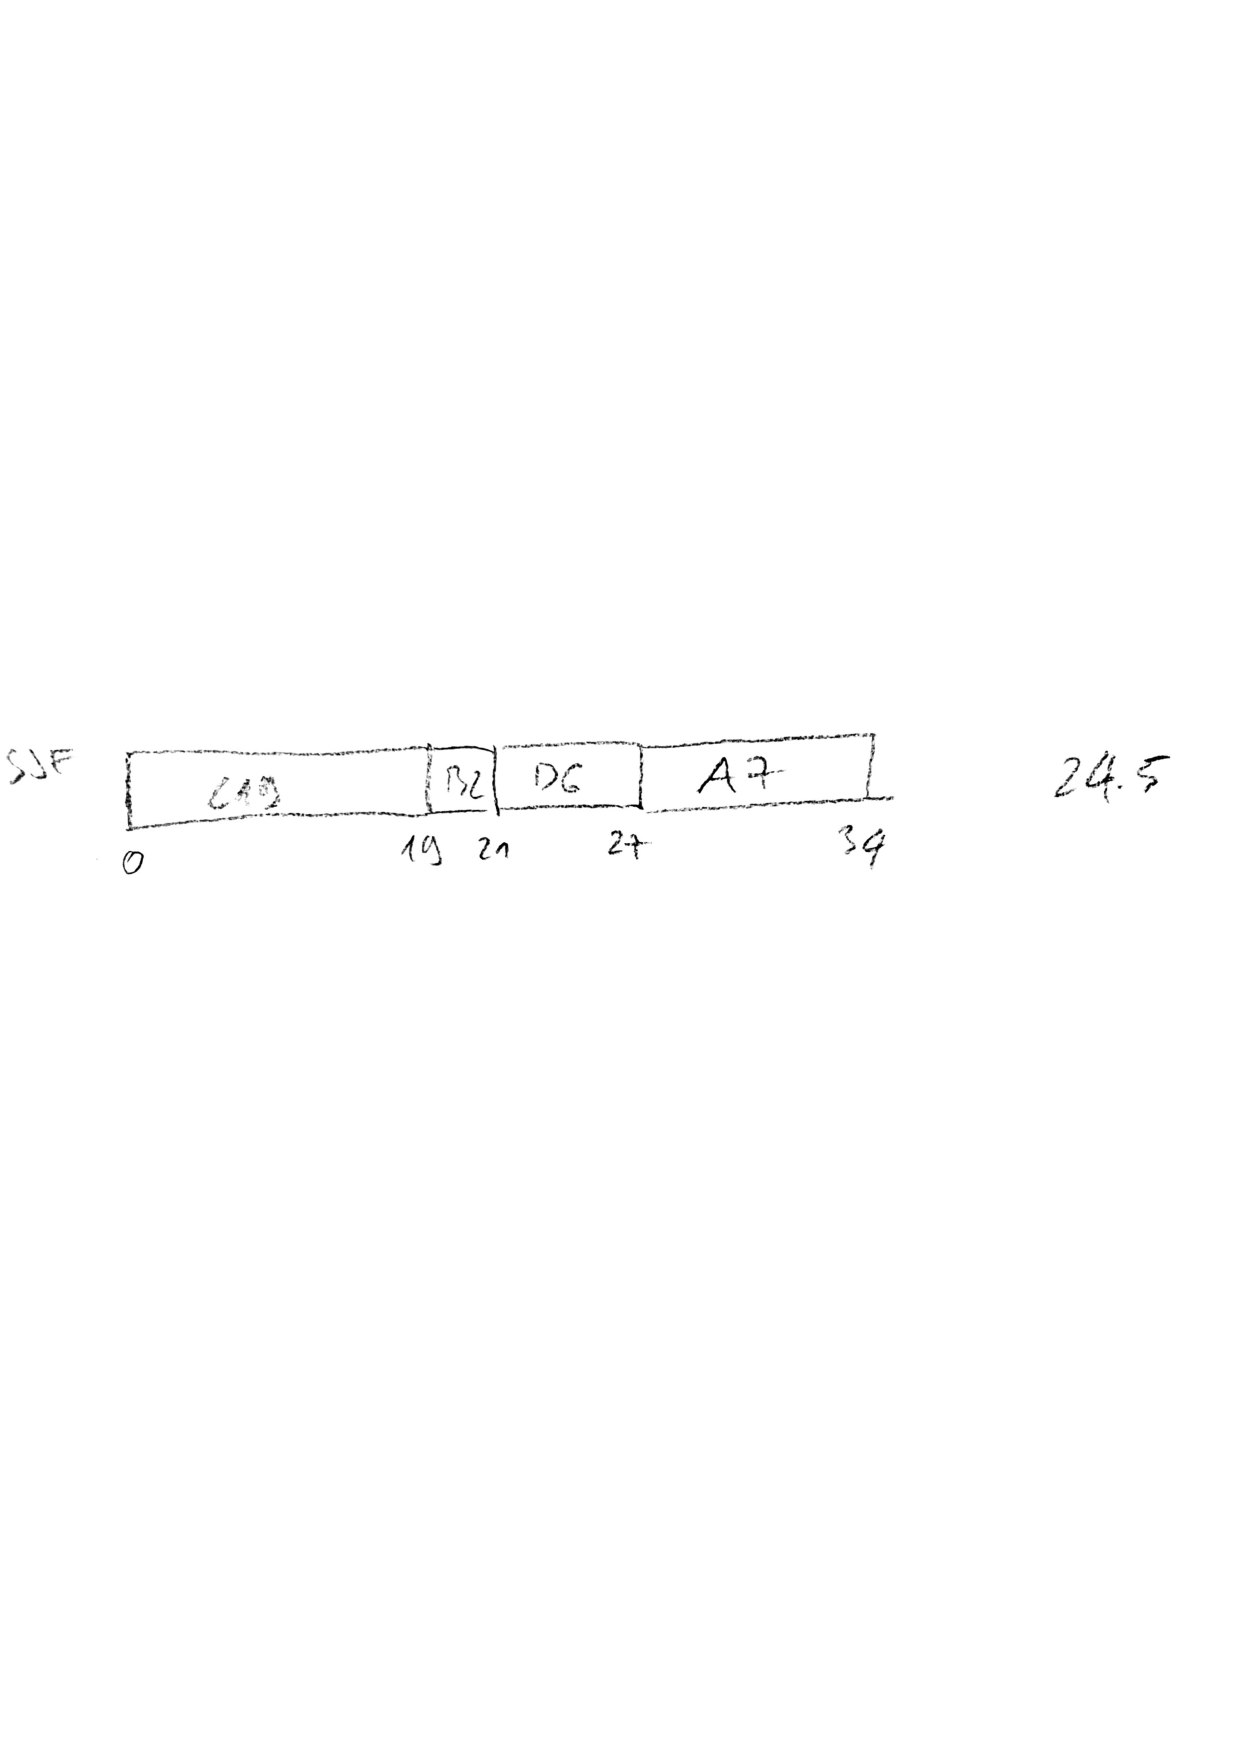
\includegraphics[width=.9\textwidth]{razvrscanje/1.7-SJF.pdf}\\
\begin{tabular}{c|cc|cc|cc}
proces & trajanje & prihod & začetek & odhod & odzivni čas & čas obdelave \\
\hline
A &   7 &  1 & 27 & 34 & 26 & 33 \\
B &   2 &  1 & 19 & 21 & 18 & 20 \\
C & 19 & 0 &  0 & 19 & 0 & 19 \\
D &   6 & 1 & 21 & 27 & 20 & 26 \\
\hline
& & & & & 16 & 24,5
\end{tabular}
\end{center}
PSJF:
\begin{center}
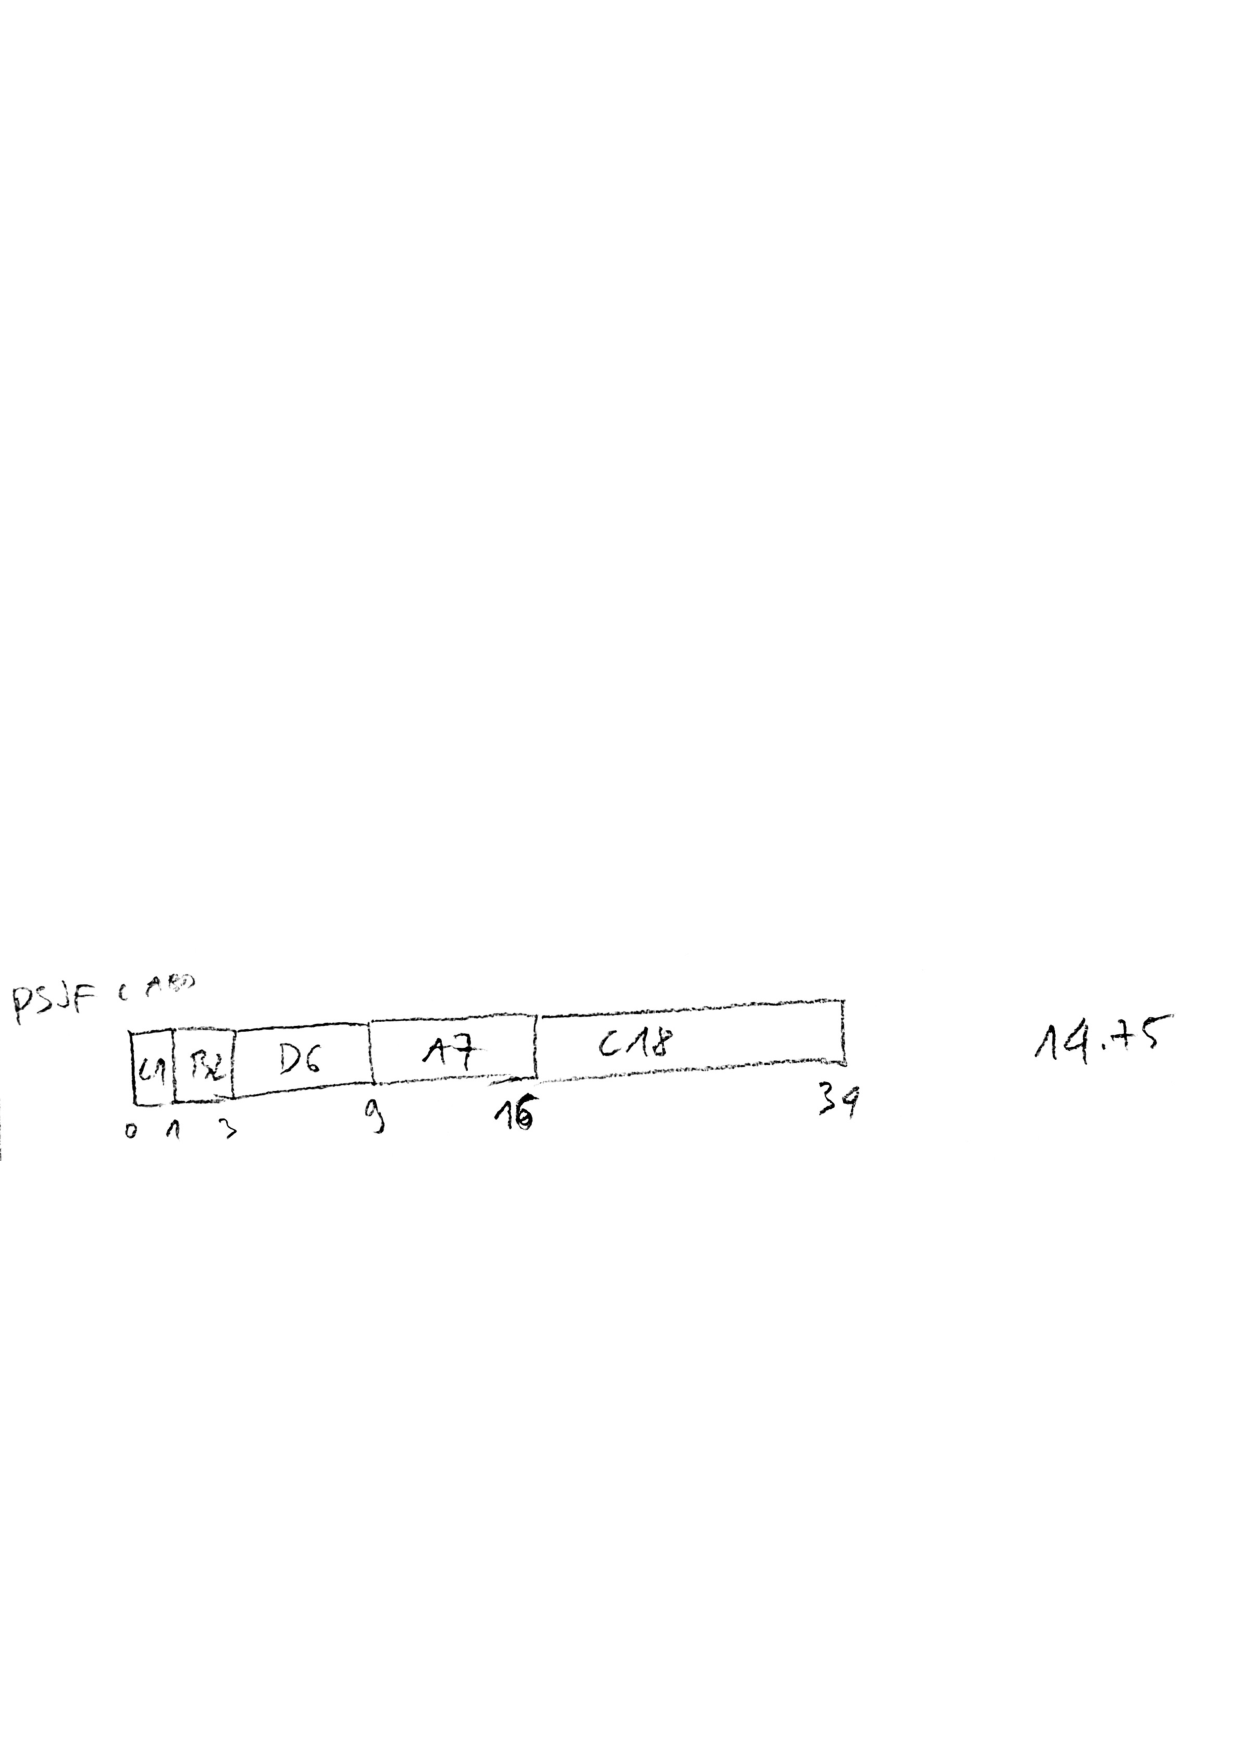
\includegraphics[width=.9\textwidth]{razvrscanje/1.7-PSJF.pdf}\\
\begin{tabular}{c|cc|cc|cc}
proces & trajanje & prihod & začetek & odhod & odzivni čas & čas obdelave \\
\hline
A &   7 &  1 & 9 & 16 & 8 & 15 \\
B &   2 &  1 & 1  & 3 & 0 & 2 \\
C & 19 & 0 & 0 & 34 & 0 & 34 \\
D &   6 & 1 & 3 & 9 & 2 & 8 \\
\hline
& & & & & 6,5 & 14,75
\end{tabular}
\end{center}
}

\section{Prednostna razvrščanja}


\begin{Exercise}
Za razvrščanje procesov v spodnji tabeli uporabi algoritem HPF, pri čemer
\begin{enumerate}
	\item uporabi sodelovano razvrščanje,
	\item uporabi prevzemno razvrščanje. 
\end{enumerate} 
\par\vspace{5pt}
{\centering
\begin{tabular}{r|ccc}
	proces & A & B & C \\
	\hline
	trajanje & 20 & 20 & 20  \\
	čas prihoda & 0 & 10 & 20 \\
	prioriteta & 1 & 2 & 3 \\
\end{tabular}\\}
\end{Exercise}
\begin{Answer}
Sodelovalno HPF razvrščanje:
\begin{center}
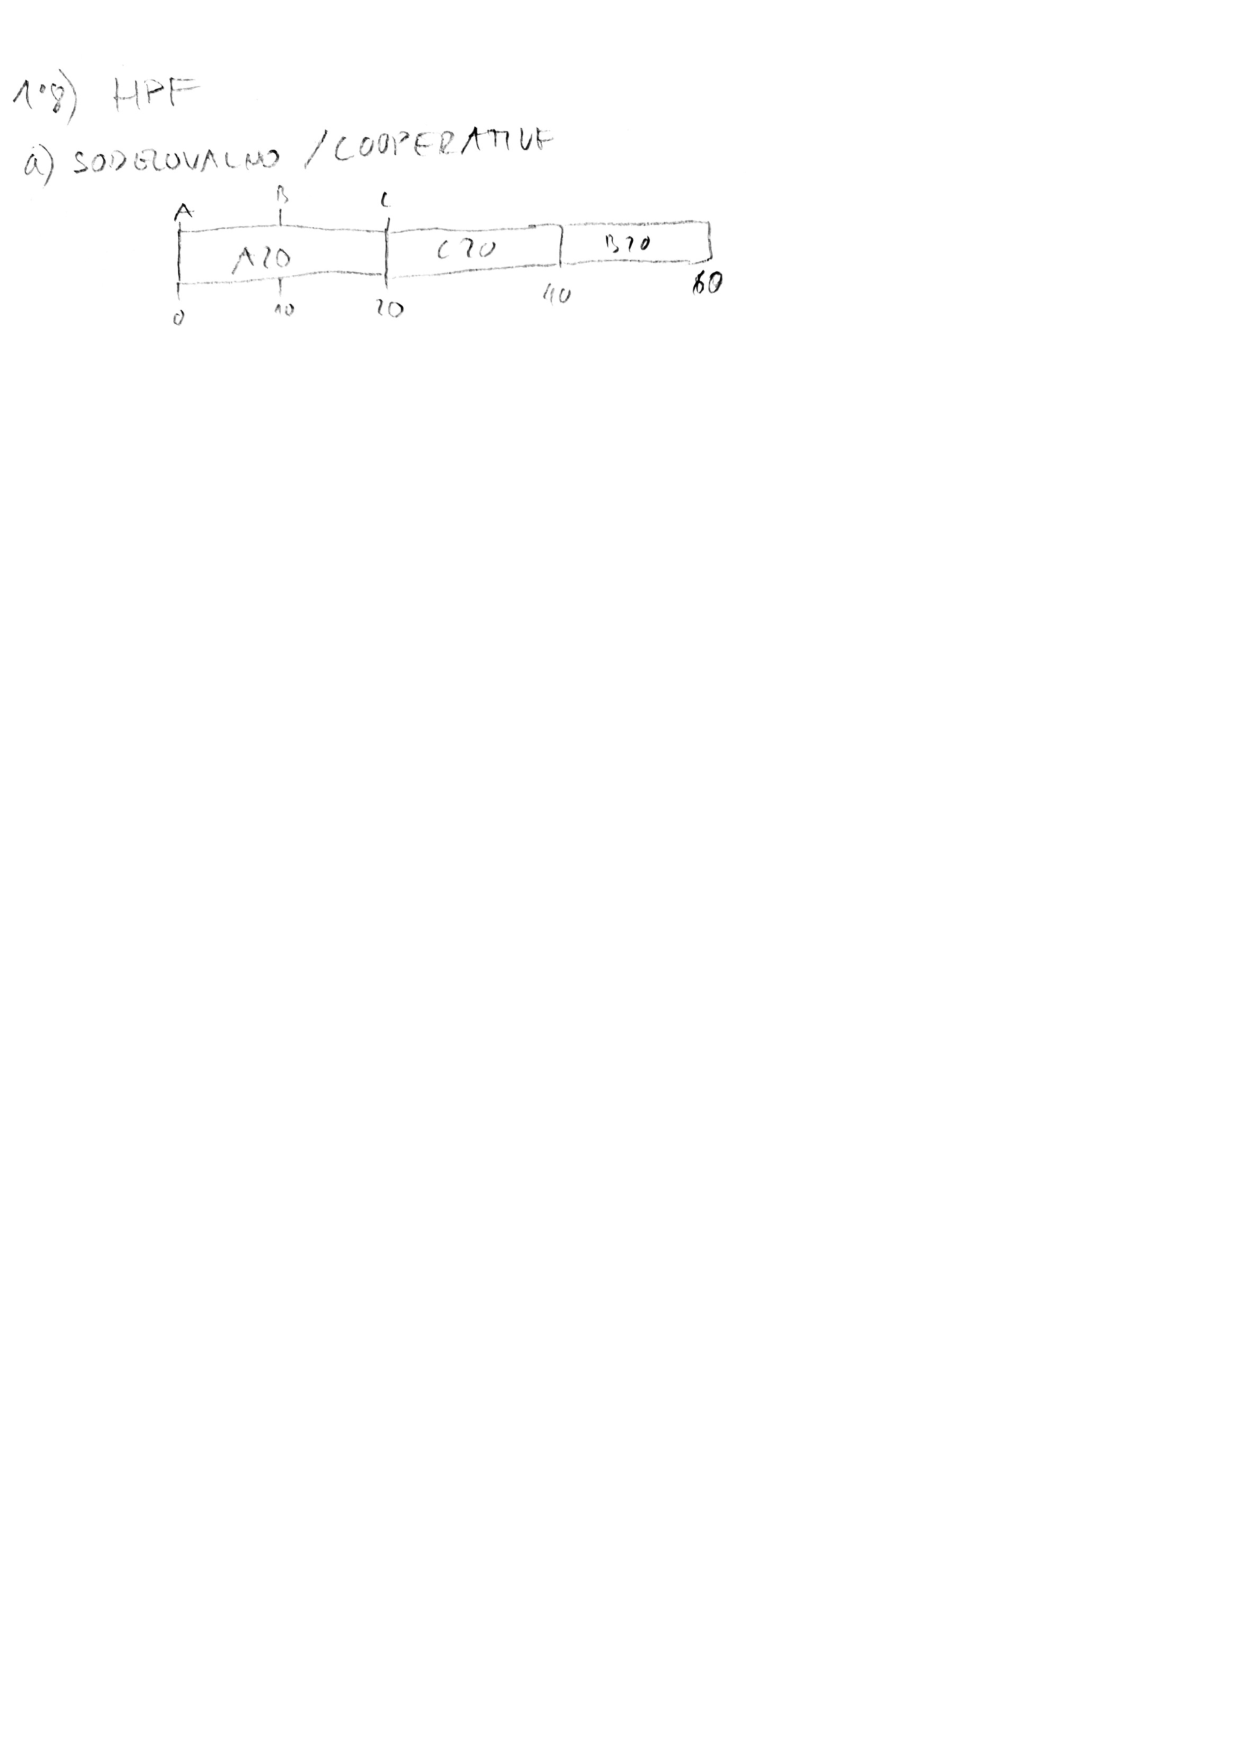
\includegraphics[width=.9\textwidth]{razvrscanje/1.8-HPF-cooperative.pdf}\\
\begin{tabular}{c|ccc|cc|cc}
proces & trajanje & prihod & prioriteta & začetek & odhod & odzivni čas & čas obdelave \\
\hline
A & 20 &  0 &  1 &   0 & 20 & 0 & 20 \\
B & 20 & 10 & 2 & 40 & 60 & 30 & 50 \\
C & 20 & 20 & 3 & 20 & 40 & 0 & 20 \\
\hline
& & & & & & 10 & 30
\end{tabular}
\end{center}
Prevzemno HPF razvrščanje:
\begin{center}
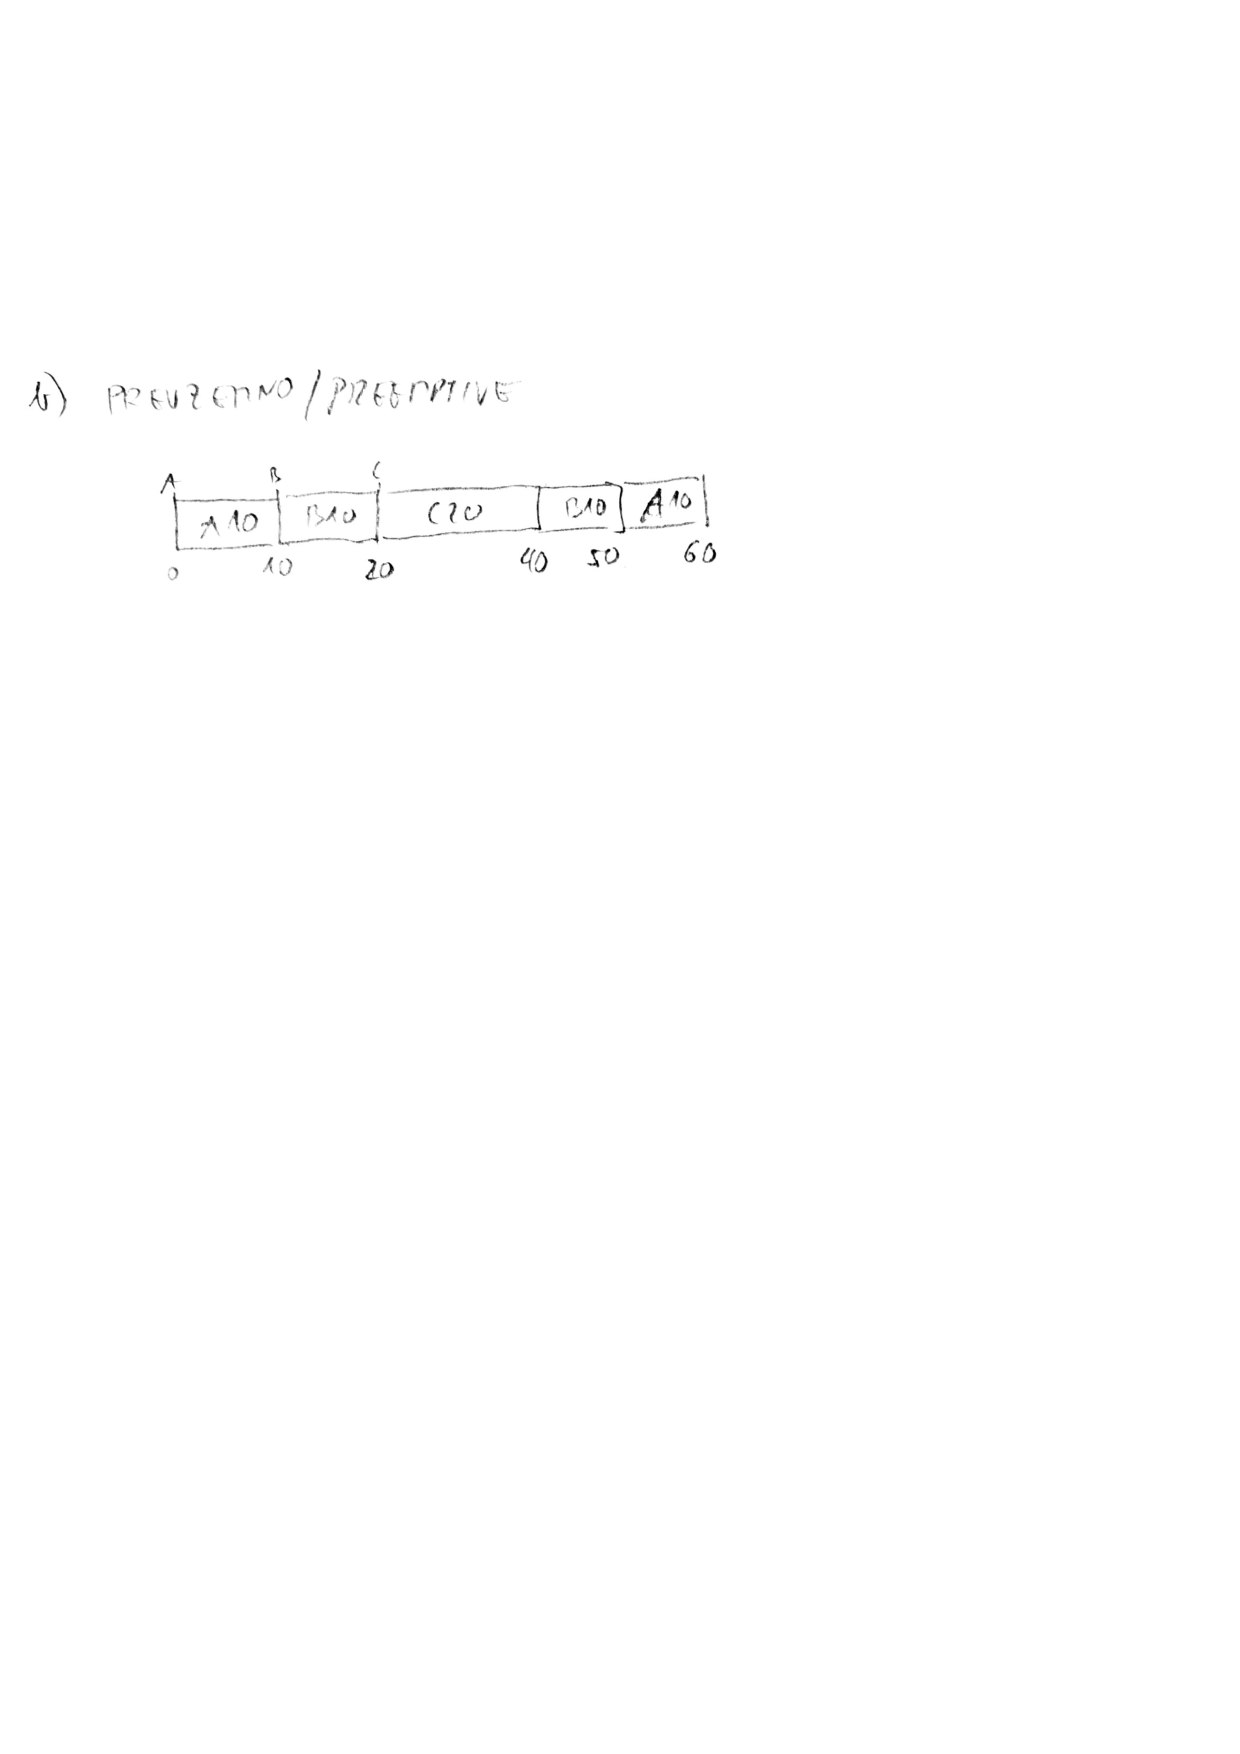
\includegraphics[width=.9\textwidth]{razvrscanje/1.8-HPF-preemptive.pdf}\\
\begin{tabular}{c|ccc|cc|cc}
proces & trajanje & prihod & prioriteta & začetek & odhod & odzivni čas & čas obdelave \\
\hline
A & 20 &  0 &  1 &   0 & 60 & 0 & 60 \\
B & 20 & 10 & 2 & 10 & 50 & 0 & 40 \\
C & 20 & 20 & 3 & 20 & 40 & 0 & 20 \\
\hline
& & & & & & 0 & 40
\end{tabular}
\end{center}
\end{Answer}


\exe{Procesi A, B in C imajo 10, 20 in 40 prepustnic zaporedoma. Razvrščevalni algoritem je izbral prepustnice št. 15, 5, 10, 42, 9, 66. Zapiši vrstni red, ki ustreza izbranimi prepustnicam. Prepustnice številčimo od 0 naprej.}
\ans{Vrstni red: B,A,B,C,A,C
\begin{center}
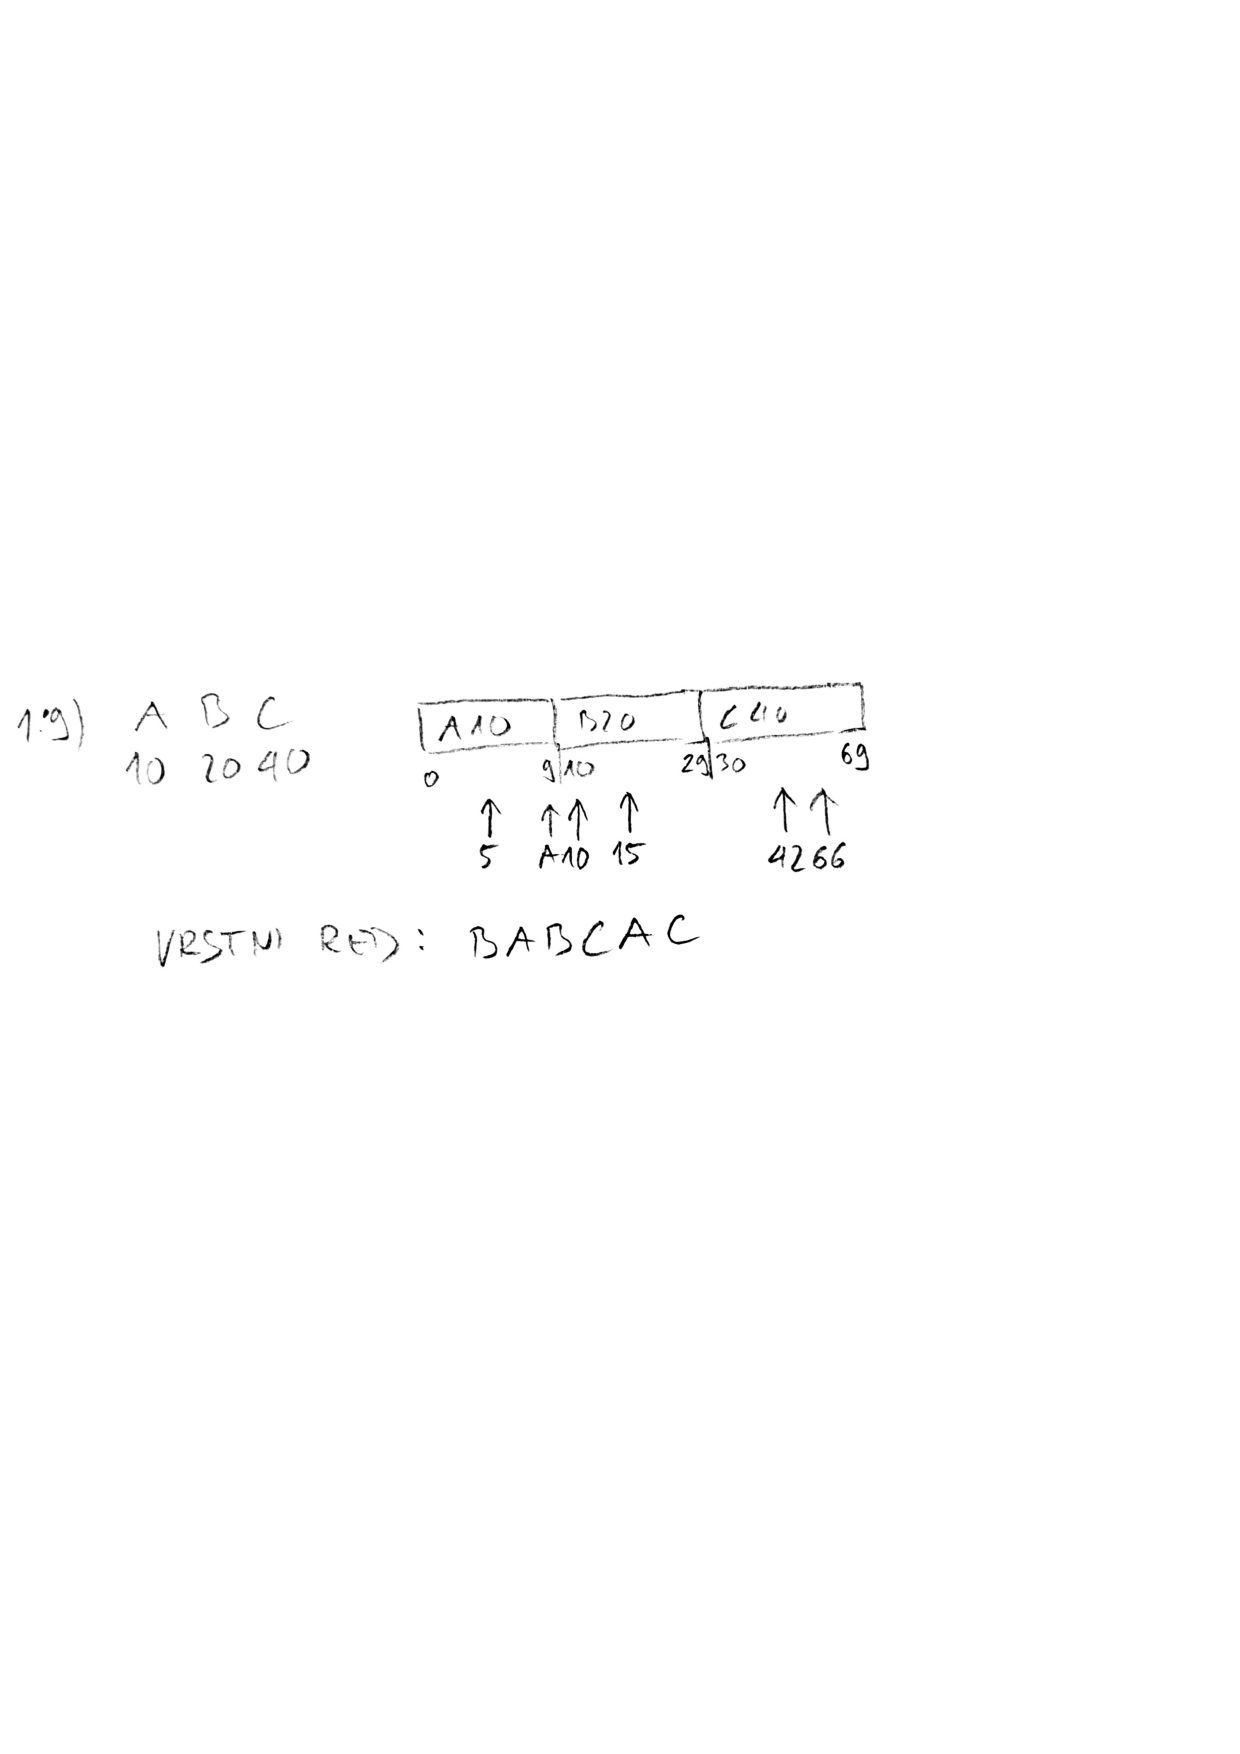
\includegraphics[width=.9\textwidth]{razvrscanje/1.9-tickets.pdf}
\end{center}
}


\exe{Procesi A, B in C imajo dolžine korakov 10, 15 in 30 zaporedoma. Uporabi koračno razvrščanje in zapiši prvih 10 izbranih procesov, pri čemer predpostavljaj \vic{neskončno} trajanje procesov.}
\ans{A,B,C,A,B,A,A,B,C, nato se vse skupaj ponovi neskončnokrat. Časovna rezina je lahko poljubna.
\begin{center}
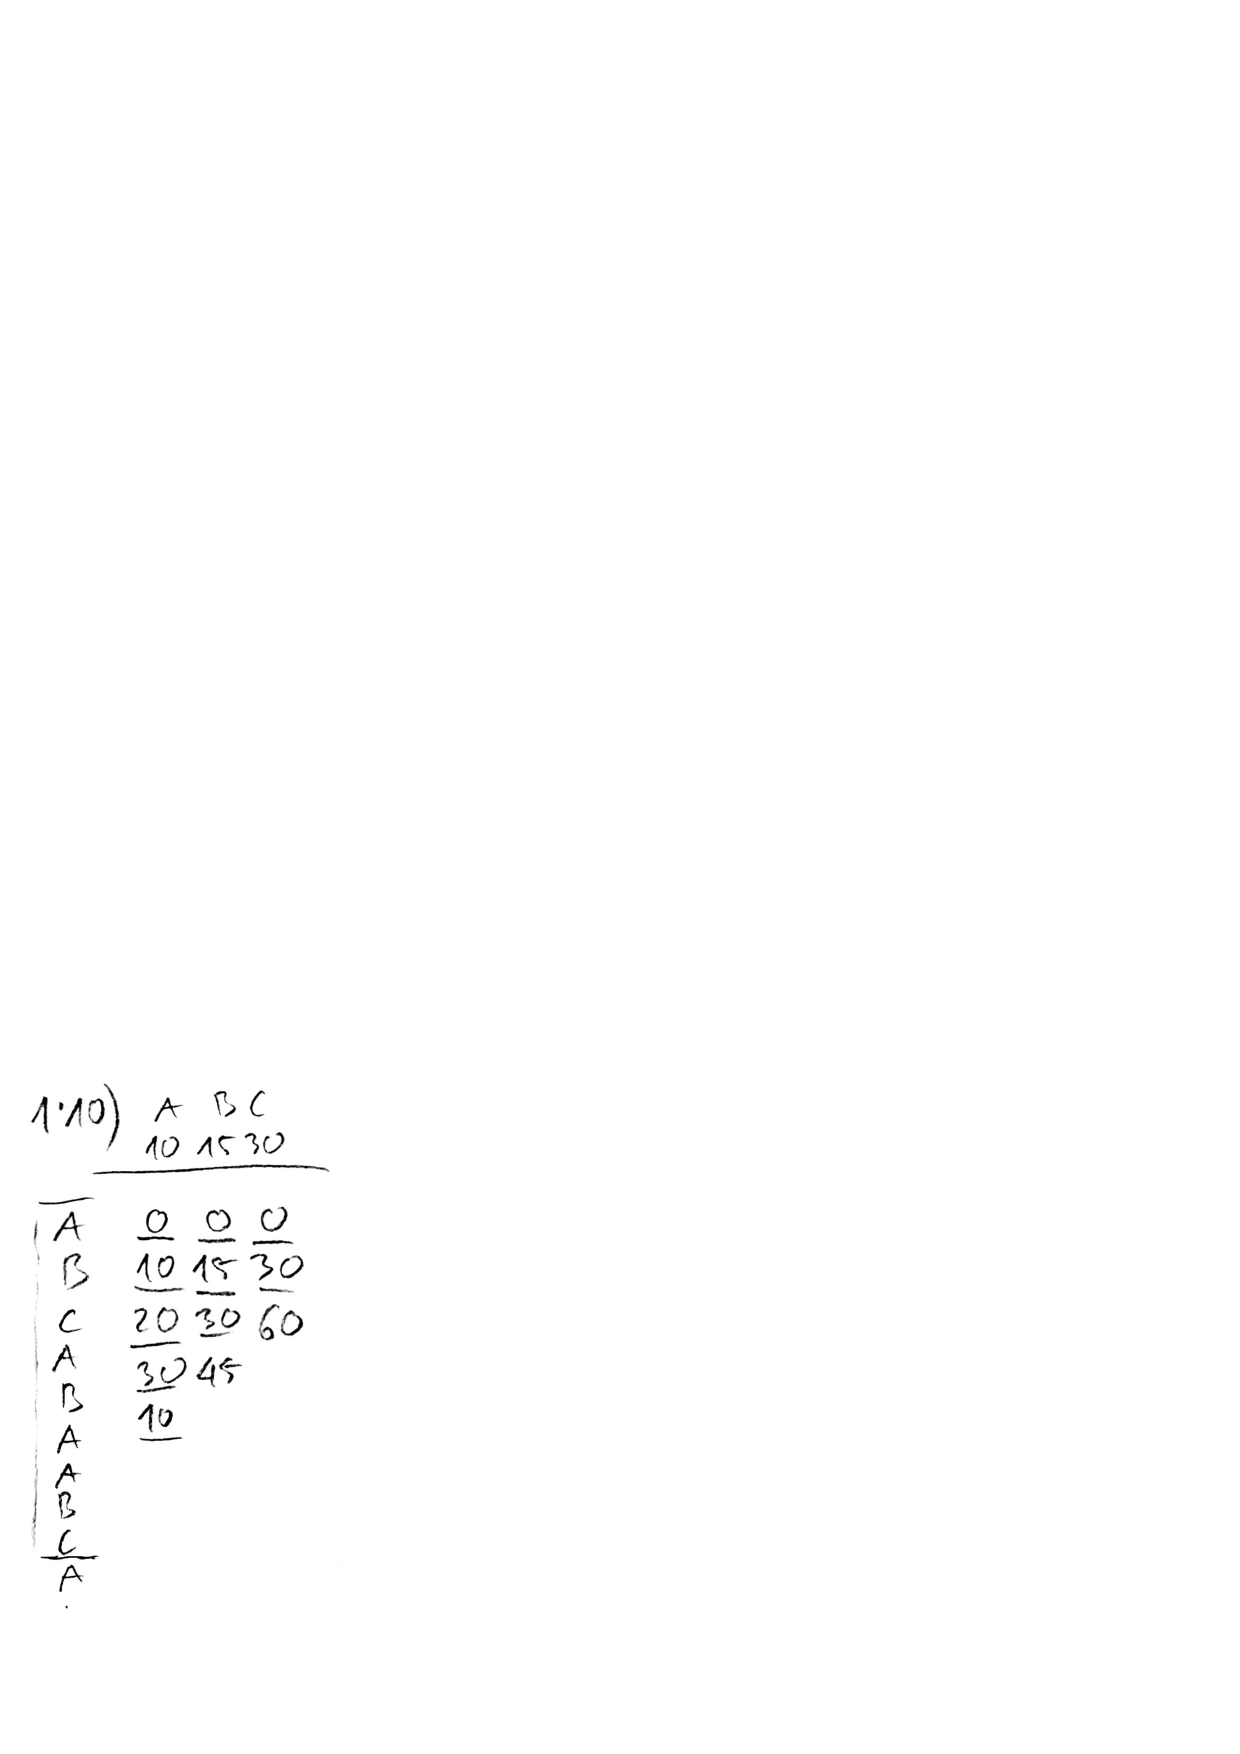
\includegraphics[width=.4\textwidth]{razvrscanje/1.10-stride.pdf}
\end{center}
}


\exe{Procesi A, B in C imajo dolžine korakov 10, 15 in 30 zaporedoma, njihovo trajanje pa je 40, 20, 30, zaporedoma. Uporabi koračno razvrščanje s časovno rezino 10 in zapiši prvih 10 izbranih procesov.}
\ans{A,B,C,A,B,A,A,C,C
\begin{center}
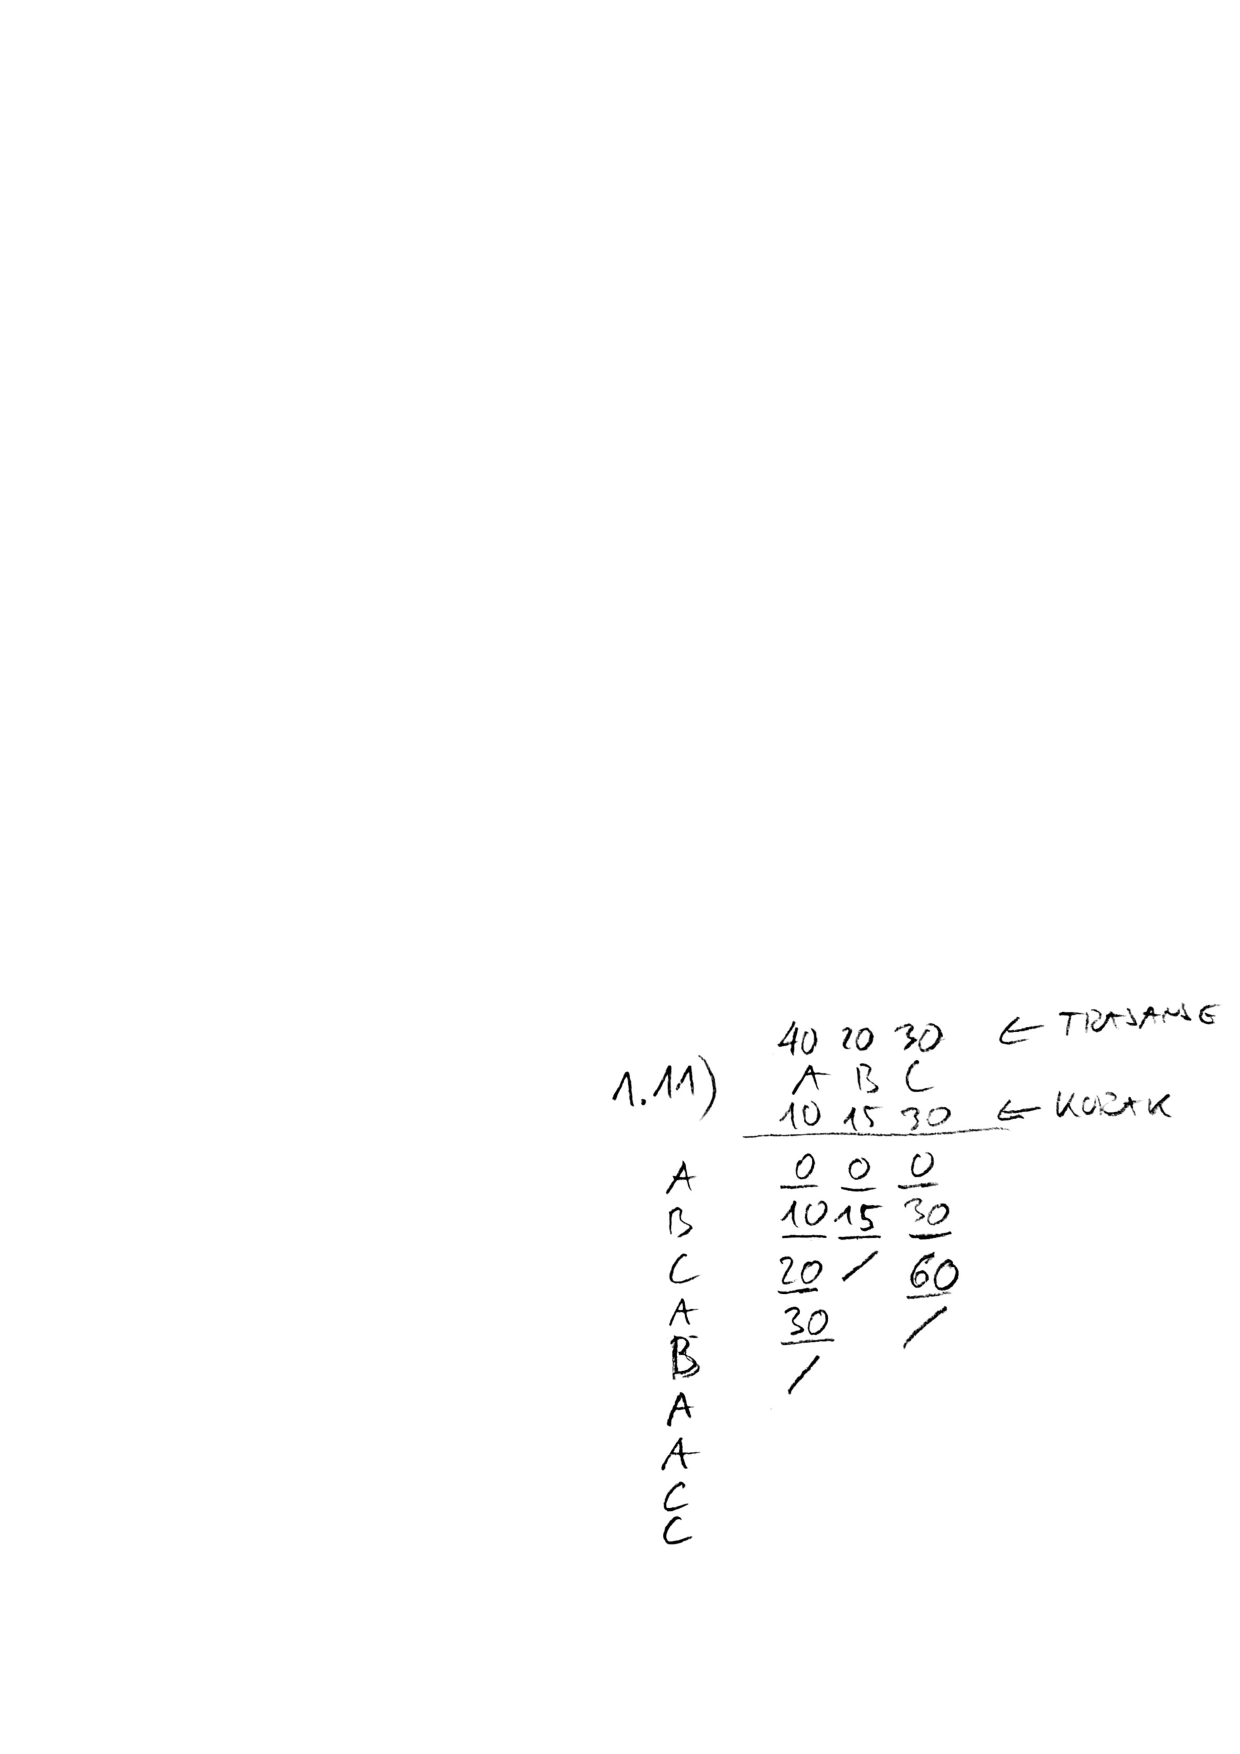
\includegraphics[width=.5\textwidth]{razvrscanje/1.11-stride.pdf}
\end{center}
}


\section{Ocenjevanje trajanja procesov}

\intro{Trajanje procesa ocenjujemo po formuli
$$ T_i = \alpha\cdot t_i + (1-\alpha)\cdot T_{i-1}, $$
kjer je $\alpha$ faktor pozabljanja, $t_i$ zadnje trajanje procesa in $T_i$ zadnja ocena trajanja. Nova ocena trajanja procesa pa je $T_{i+1}$. Začetno oceno označimo s $T_0$.}


\begin{Exercise}
Naj bo $\alpha=0.5$ faktor pozabljanja in $T_0=5$ začetna ocena trajanja procesa. Dopolni tabelo z ocenami trajanja procesov:
\par
{\centering
	\begin{tabular}{c|cccc}
		$i$    & 1 & 2 & 3 & 4 \\ 
		\hline
		$t_i$ & 11 & 4 & 2 & 20 \\
		$T_i$ &  &  &  &  \\
	\end{tabular}\\
}
\end{Exercise}
\ans{
	\begin{tabular}{c|cccc}
	$i$    & 1 & 2 & 3 & 4 \\ 
	\hline
	$t_i$ & 11 & 4 & 2 & 20 \\
	$T_i$ & 8 & 6 & 4 & 12 \\
	\end{tabular}\\
}


\begin{Exercise}
Naj bo $\alpha=0.2$ faktor pozabljanja in $T_0=10$ začetna ocena trajanja procesa. Dopolni tabelo z ocenami trajanja procesov:
\par
{\centering
	\begin{tabular}{c|cccc}
	$i$    & 1 & 2 & 3 & 4 \\ 
	\hline
	$t_i$ & 10  & 15 & 16 & 22\\
	$T_i$ & & & & \\
	\end{tabular}\\
}
\end{Exercise}
\ans{
\begin{tabular}{c|cccc}
	$i$    & 1 & 2 & 3 & 4 \\ 
	\hline
	$t_i$ & 10  & 15 & 16 & 22\\
	$T_i$ & 10 & 11 & 12 & 14 \\
\end{tabular}\\
}


\section{Namigi in rešitve izbranih nalog}

\shipoutAnswer

%\include{zahtevnost}
%\include{podatkovne_strukture}
%\include{urejanja}
%\include{drevesa}
%\include{grafi}
%\include{metode_snovanja}
%\include{groba_sila}
%\include{deli_in_vladaj}
%\include{pozresni_algoritmi}


\end{document}
